%
% main.tex -- Paper zum Thema Datenassimilation für Lorenz-System
%
% (c) 2018 Hochschule Rapperswil
%
\chapter{Datenassimilation für das Lorenz-System\label{chapter:kalman}}
\lhead{Datenassimilation für das Lorenz-System}
\begin{refsection}
\chapterauthor{Michael Müller}

\section{Datenassimilation}
\rhead{Datenassimilation}
Die meteorologische Datenassimilation hat zur Aufgabe, Anfangszust"ande f"ur die numerische Wettervorhersage (analysis or filtering mode), Klimaprojektionen (forecasting or predicting mode) oder Untersuchungen am vergangenen Erdklima (reanalysis or smoothing mode) zur Verf"ugung zu stellen, die r"aumlich und zeitlich unvollst"andig vorliegen. Die Datenassimilation nutzt hierzu direkte und indirekte Messungen der Atmosph"are in Kombination mit berechneten Modellzust"anden, um daraus einen in sich stimmigen Gesamtzustand zu ermitteln. Die Ermittlung des Zustandes der Atmosph"are erfolgt in regelm"assigen zeitlichen Abst"anden, dem sogenannten Datenassimilations-Zyklus, durch welchen eine verl"assliche Bestimmung der atmosph"arischen Gr"ossen wie Druck oder Temperatur m"oglich wird.

\section{Kalmanfilter}
\rhead{Kalmanfilter}
Ein Werkzeug der Datenassimilation ist der Kalmanfilter mit seinen diversen Abwandlungen. In diesem Kapitel wird der Extended Kalmanfilter genauer erkl"art und auf die n"otigen Parameter eingegangen. Extended bezeichnet hier eine Erweiterung des Kalmanfilters auf nicht-lineare dynamische Systeme, wie in diesem Beispiel dem Lorenz-Modell aus dem Jahre 1963 (LM63). Er wurde im Zuge der Apollo Mission von Stanley F. Schmidt entwickelt und zur Navigation im Weltraum angewendet.\\

Der Kalmanfilter ist ein rekursives Verfahren zur Filterung von Datens"atze, bei dem  der zuk"unftige Datenpunkt als Linearkombination der Beobachtung und einer Vorhersage durch ein mathematisches Systemmodell gesch"atzt wird. Voraussetzung f"ur die Beobachtung ist die Messung mindestens einer Systemvariablen mit zugeh"origer Varianz. F"ur das Modell ist eine Matrix n"otig, die aus dem alten Zustand auf den neuen schliessen l"asst.\\

\subsection{Allgemeine Funktionsweise}
\rhead{Allgemeine Funktionsweise}

Die Struktur des Kalmanfilter-Algorithmus erlaubt eine Echtzeitfilterung und macht ihn so f"ur diverse Anwendungen interessant.\\
\\
Der Algorithmus besteht aus folgender Schrittfolge:\\
1) Die Vorhersage wird sowohl f"ur den folgenden Datenpunkt sowie dessen Kovarianz durchgef"uhrt, wobei das \(\phi\) die Transformationsmatrix ausdr"uckt, wie vom jetzigen Zustand auf den n"achsten geschlossen werden kann. Die Notation \(\hat{x}_{k+1|k}\) bedeutet die Sch"atzung von \(x\) zum Zeitpunkt \(k\) f"ur den n"achsten Zeitpunkt \(k+1\) .\\
\[\hat{x}_{k+1|k} = \phi\hat{x}_{k}\]
\[P_{k+1|k}=\phi_{k}P_{k}\phi_{k}^{t}+Q_{k}\]
2) Kalmanfaktor\\
Der Kalmanfaktor \(K\), gewichtet in Abh"angigkeit der beiden Fehlerkovarianzen die Beobachtung oder das Systemmodell st"arker. Dabei l"ost der Algorithmus das Problem optimal,so dass sich f"ur die sp"ater korrigierte Vorhersage das Minimum der resultierenden Kovarianz ergibt.\\
\[K_{k}=P_{k|k-1}H^{t}_{k}(H_{k}P_{k|k-1}H^{t}_{k}+R_{k})^{-1}   \]
3) Korrektur\\
Die Vorhersage wird nun mit dem Kalmanfaktor und der Messung korrigiert. In der folgenden Beschreibung ist die Gewichtung durch den Kalmanfaktor in der Matrixschreibweise zu erkennen. Dasselbe Vorgehen gilt f"ur die Kovarianzmatrix $P$.\\
\begin{align*}
\hat{x}_{k}&=(I-K_{k}H_{k})\hat{x}_{k|k-1}+K_{k}z_{k}\\
P_{k}&=(I-K_{k}H_{k})P_{k|k-1}(I-K_{k}H_{k})^{t}+K_{k}R_{k}K^{t}_{k}  \end{align*}
\\
\(H\) ist die Messmatrix und gibt an, welche Komponenten, mit allf"alliger Verst"arkung, gemessen werden k"onnen. \(R_{k}\) und \(Q_{k}\) sind die Kovarianzen der Messung und des Systems. Die Simulation wie auch die Messung sind mit einem normalverteilten Fehler, \(u_{k} \text{ und } w_{k}\),"uberlagert. F"ur die Messung sowie das vorangehende Systemmodell gilt folgendes:

\begin{align*}
z_{k}&=H_{k}x_{k}+w_{k} \text{, mit } w_{k}\sim N\langle0,\sigma^{2}\rangle\\
R_{k}&=E(w_{k}w^{t}_{k})\\
x_{k}&=\phi_{k-1}x_{k-1}+u_{k} \text{, mit } u_{k}\sim N\langle0,\sigma^{2}\rangle\\ 
Q_{k}&=E(u_{k}u^{t}_{k})
\end{align*}

\subsection{Anwendung auf das Lorenz-System}
\rhead{Anwendung auf das Lorenz-System}
Als Anwendungsbeispiel f"ur den Kalmanfilter nun die Parameter mit dem LM63. Die Fehlerkovarianzen sind konstant und haben bei vollst"andig erfassbaren Messwerten folgende Form.
\[R=\begin{pmatrix}
\sigma^{2}_{x} & 0 & 0 \\ 
0 & \sigma^{2}_{y} & 0 \\ 
0 & 0 & \sigma^{2}_{z}
\end{pmatrix}  \text{, }
Q=\begin{pmatrix}
\sigma^{2}_{x} & 0 & 0 \\ 
0 & \sigma^{2}_{y} & 0 \\ 
0 & 0 & \sigma^{2}_{z}
\end{pmatrix} 
\]
Die Messmatrizen, die f"ur diese Arbeit Verwendung finden, sind unten dargestellt. Die Einheitsmatrix $H_{1}$ misst zum Beispiel jeden der drei Eintr"age des Lorenz Systems $\begin{pmatrix}x & y & z
\end{pmatrix}$. Die zweite Messmatrix misst den x-Eintrag nur als Kombination von x und y sowie den y-Eintrag als Kombination von y und z, was oft die Realit"at widerspiegelt, wo Messgr"ossen nicht direkt gemessen werden k"onnen. $H_{3}$ und $H_{4}$ als anspruchsvolle Beispiele f"ur den Filter, wo Messwerte fehlen und damit f"ur je eine Variable keine Korrekturm"oglichkeit besteht.
\[H_{1}=\begin{pmatrix}
1 & 0 & 0 \\ 
0 & 1 & 0 \\ 
0 & 0 & 1
\end{pmatrix} 
\text{, }
H_{2}=\begin{pmatrix}
1 & 1 & 0 \\ 
0 & 1 & 1 \\ 
\end{pmatrix}
\text{, }
H_{3}=\begin{pmatrix}
1 & 0 & 0 \\ 
0 & 1 & 0 \\ 
\end{pmatrix}
\text{, }
H_{4}=\begin{pmatrix}
1 & 0 & 0 \\  
0 & 0 & 1
\end{pmatrix}
\]
Der Messwert mit $H_{3}$ sieht dann zum Beispiel wie folgt aus:
\[\hat{z}_{k}=
\begin{pmatrix}
\hat{x} \\
\hat{y} \\
\end{pmatrix}= 
\underbrace{\begin{pmatrix}
1 & 0 & 0  \\
0 & 1 & 0
\end{pmatrix}}_{H_{3}}
\begin{pmatrix}
x \\
y \\
z \\
\end{pmatrix}+
\underbrace{\begin{pmatrix}
\sigma_{x} & 0 \\
0 & \sigma_{y}
\end{pmatrix}}_{Fehler R}
\]
Eine Schwierigkeit stellt die Herleitung vom $\phi$ f"ur den Filter dar. Als Einf"uhrung ein kurzes Beispiel aus der translatorischen Bewegungsgleichung zur Positionsbestimmung.
\[
\underbrace{\begin{pmatrix}
s_{k+1|k} \\ 
v_{k+1|k} \\ 
a_{k+1|k}
\end{pmatrix}}_{\hat{x}_{k+1}}
=
\underbrace{\begin{pmatrix}
 1 & \Delta t & \frac{1}{2}\Delta t^{2} \\ 
 0 & 1 & \Delta t \\ 
 0 & 0 & 1
 \end{pmatrix}}_{\phi}
\underbrace{\begin{pmatrix}
   s_{k} \\ 
   v_{k} \\ 
   a_{k}
   \end{pmatrix}}_{\hat{x}_{k}}
\]
Eine Matrix $\phi$ f"ur das nicht-lineare chaotische System wie das LM63 kann nicht auf diese  Weise aufgestellt werden. Eine M"oglichkeit ist die Abh"angigkeit von Anfangsbedingungen, daher wie stark "andert sich der Zielwert, wenn die Anfangsbedingung um ein $\Delta x_{0}$ ver"andert wird. Wie stark deren Einfluss sein kann, zeigt symbolisch Abbildung \ref{skript:AblnachAnf}.

\begin{figure}
\centering
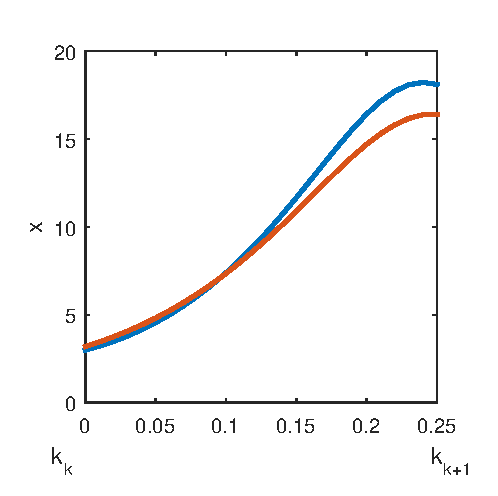
\includegraphics[width=3in]{kalman/figures/ablnachAnf2.eps}
\caption{Ableiten nach den Anfangsbedingungen}
\label{skript:AblnachAnf}
\end{figure}

W"ahrend des Datenassimilations-Zyklus wird das Systemmodell mit den Anfangsbedingungen sowie dem $\phi$ mittels folgender Formel gel"ost und integriert:
\[
\frac{d}{dt}\begin{pmatrix}
x \\ 
y \\ 
z \\ 
\textbf{J}
\end{pmatrix}=
\begin{pmatrix}
f(x,y,z) \\ 
\textbf{F}(x,y,z)\textbf{J}
\end{pmatrix} 
\text{, mit Anfangsbedingung }
X(0)=\begin{pmatrix}
x_{0}\\
y_{0}\\
z_{0}\\ 
\textbf{E}
\end{pmatrix} 
\]
\[
\text{ mit $F$ als Jakobische Matrix des LM63 }F(x,y,z) = \begin{pmatrix}
-\sigma & \sigma & 0 \\ 
\rho-z & -1 & -x \\ 
y & x & -\beta
\end{pmatrix} 
\]
\textbf{J} und \textbf{E} sind $3\times3$ Matrizen, die spaltenweise in den Vektor eingef"ullt wurden. $f(x,y,z)$ ist die rechte Seite des LM63. Der gel"oste Vektor hat dann f"ur unser System folgende Form:
\[
X_{k}=\begin{pmatrix}
x \\ 
y \\ 
z \\  
J_{11} \\ 
J_{12} \\ 
J_{13} \\ 
J_{21} \\ 
J_{22} \\ 
J_{23} \\ 
J_{31} \\ 
J_{32} \\
J_{33} 
\end{pmatrix}
\]
Die Herleitung dieser Formeln ist im Buch Differentialgleichungen im Kapitel 2.1.5 Ableitung nach der Anfangsbedingung aus dem mathematischen Seminar im FS2016 zu finden. Die Eintr"age aus $X_{k}$ von 4-12 werden nun wieder spaltenweise in eine 3x3 Matrix umgewandelt, welche nun unser gesuchtes $\phi$ ist.\\

\subsection{Parameter und Initialisierung}
\rhead{Parameter und Initialisierung}
Die Werte f"ur die charakteristischen Parameter des Lorenz-System, unter deren ein chaotisches Verhalten m"oglich ist, werden auch hier verwendet.\\
\[
\sigma=10 \text{ , } \beta=8/3 \text{ , }\rho=28
\]
Der Startwert $x_{0}$ ist vom Standardwert $\begin{pmatrix}
3 & 15 & 1
\end{pmatrix}^{t}$ verschieden, um das chaotische Verhalten schneller herbeizuf"uhren und Rechenzeit einzusparen. Gezeigt wird auch nur jeweils der Ausschnitt zwischen $t = 5$ und $t=10$, da an der Stelle das chaotische Verhalten ausgepr"agt vorhanden ist. $P_{0}$, als Startwert f"ur die Varianz der Simulation, wird zur Sicherheit gross gew"ahlt. Dies hat f"ur die Berechnung keinen signifikanten Einfluss, da der Algorithmus den Wert zeitnah korrigiert. $J$ wird mit der Einheitsmatrix initialisiert und dient der Berechnung des $\phi$. Diese Matrix wird "uber mehrere Zwischenschritte, mit Vorhersage und Korrektur, bis zum Zeitpunkt $t_{k+1}$ integriert.
\[x_{0}=\begin{pmatrix}
3 \\ 
5 \\ 
5
\end{pmatrix} 
\text{, }
P_{0}=\begin{pmatrix}
10 & 0 & 0 \\ 
0 & 10 & 0 \\ 
0 & 0 & 10
\end{pmatrix} 
\text{, }
J=\begin{pmatrix}
1 & 0 & 0 \\ 
0 & 1 & 0 \\ 
0 & 0 & 1
\end{pmatrix} 
\]
Zuf"allige St"orsignale in der Messung oder in die Simulation werden keine eingebaut, da aufgrund der starken Vereinfachungen und Transformationen bis hin zum Lorenzmodell aus einem urspr"unglichen Messfehler (z.B. $\pm1^\circ C$) kein R"uckschluss mehr m"oglich w"are.

\subsection{Anmerkungen zur Kovarianzmatrix und dem Kalmanfaktor}
\rhead{Anmerkungen zur Kovarianzmatrix und dem Kalmanfaktor}
Da $P_{k+1|k}=f(\phi, Q)$, $K=f(P,H,R)$ sowie $P_{k}=f(K,H,R)$ im Falle der Positionsbestimmung Konstanten sind, m"ussen sie nicht in jedem Zyklus neu berechnet werden und k"onnen als Konstanten einprogrammiert werden. Im diesem Fall ist das $\phi$ eine Variable, weshalb die $K$ und $P$ auch Variablen sind und jeweils berechnet werden m"ussen. Zwei Beispiele sind in der Abbildung \ref{skript:Kovarianz} dargestellt. Es ist sowohl eine deutliche Abnahme der Genauigkeit sowie deutlich st"arkere Fluktuationen von $H_{1}$ zu $H_{2}$ erkennen.

\begin{figure}
\centering
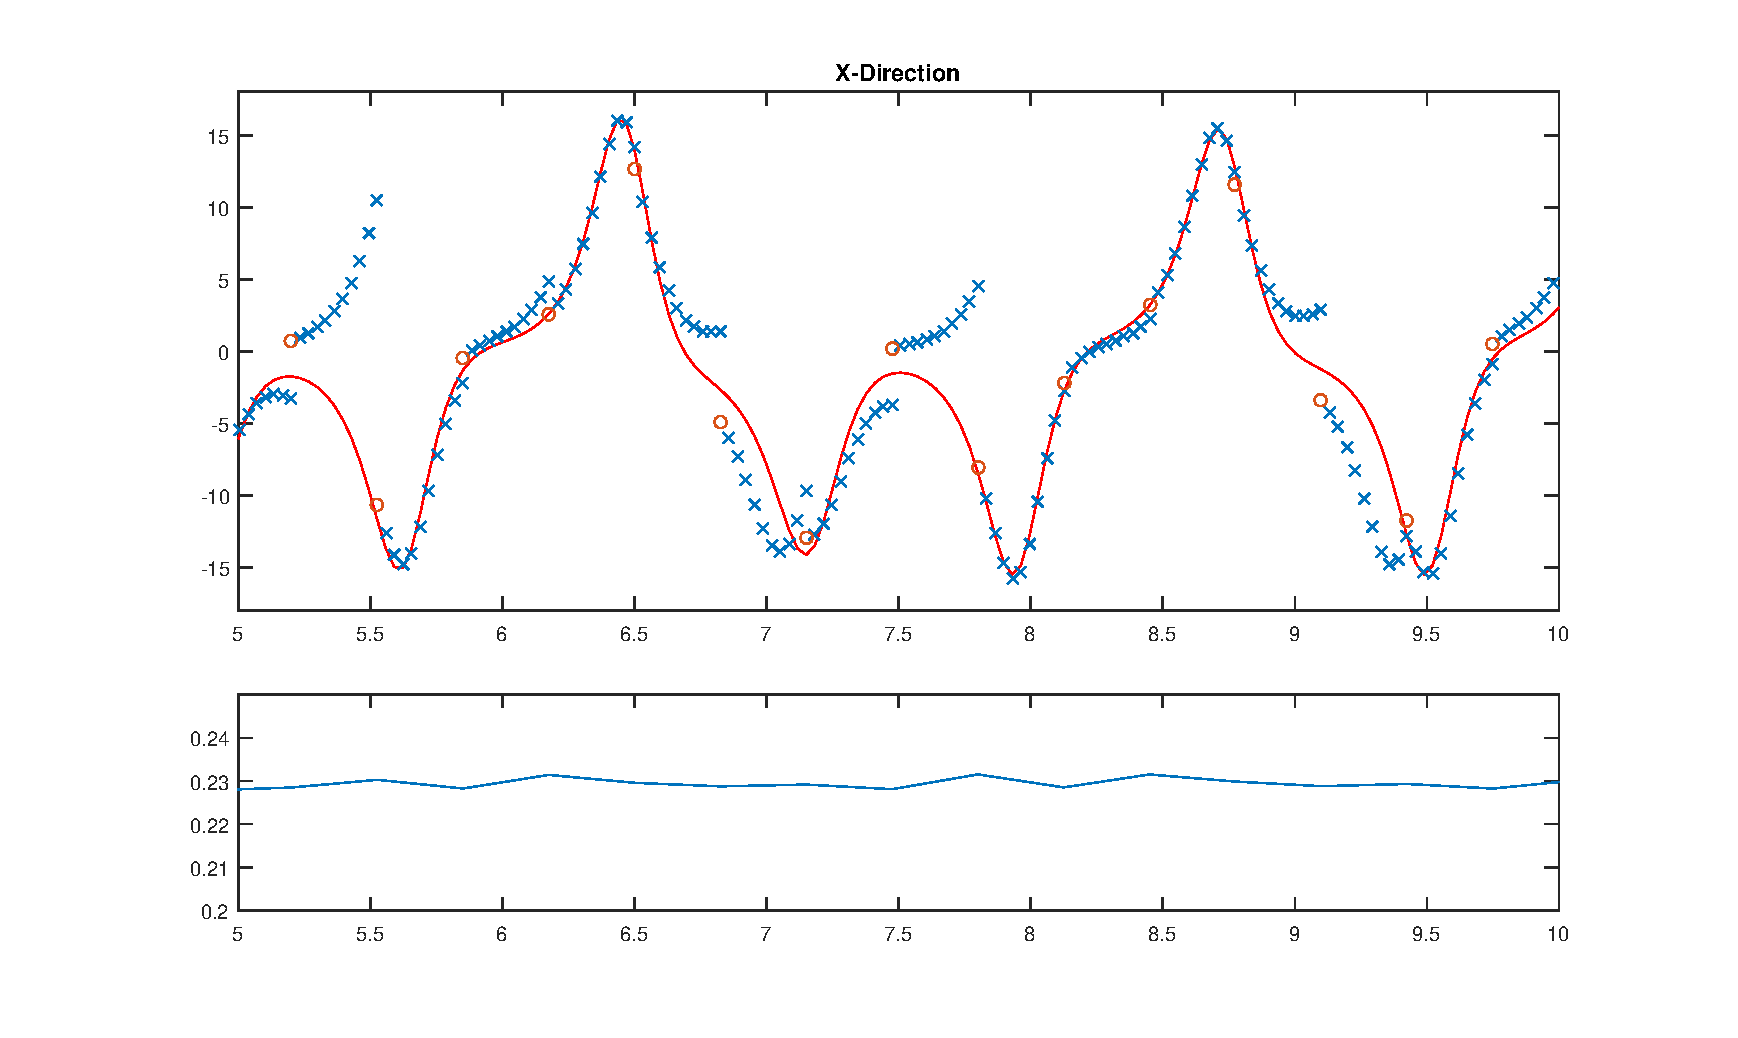
\includegraphics[width=\hsize]{kalman/figures/H1R10S2XP.eps}
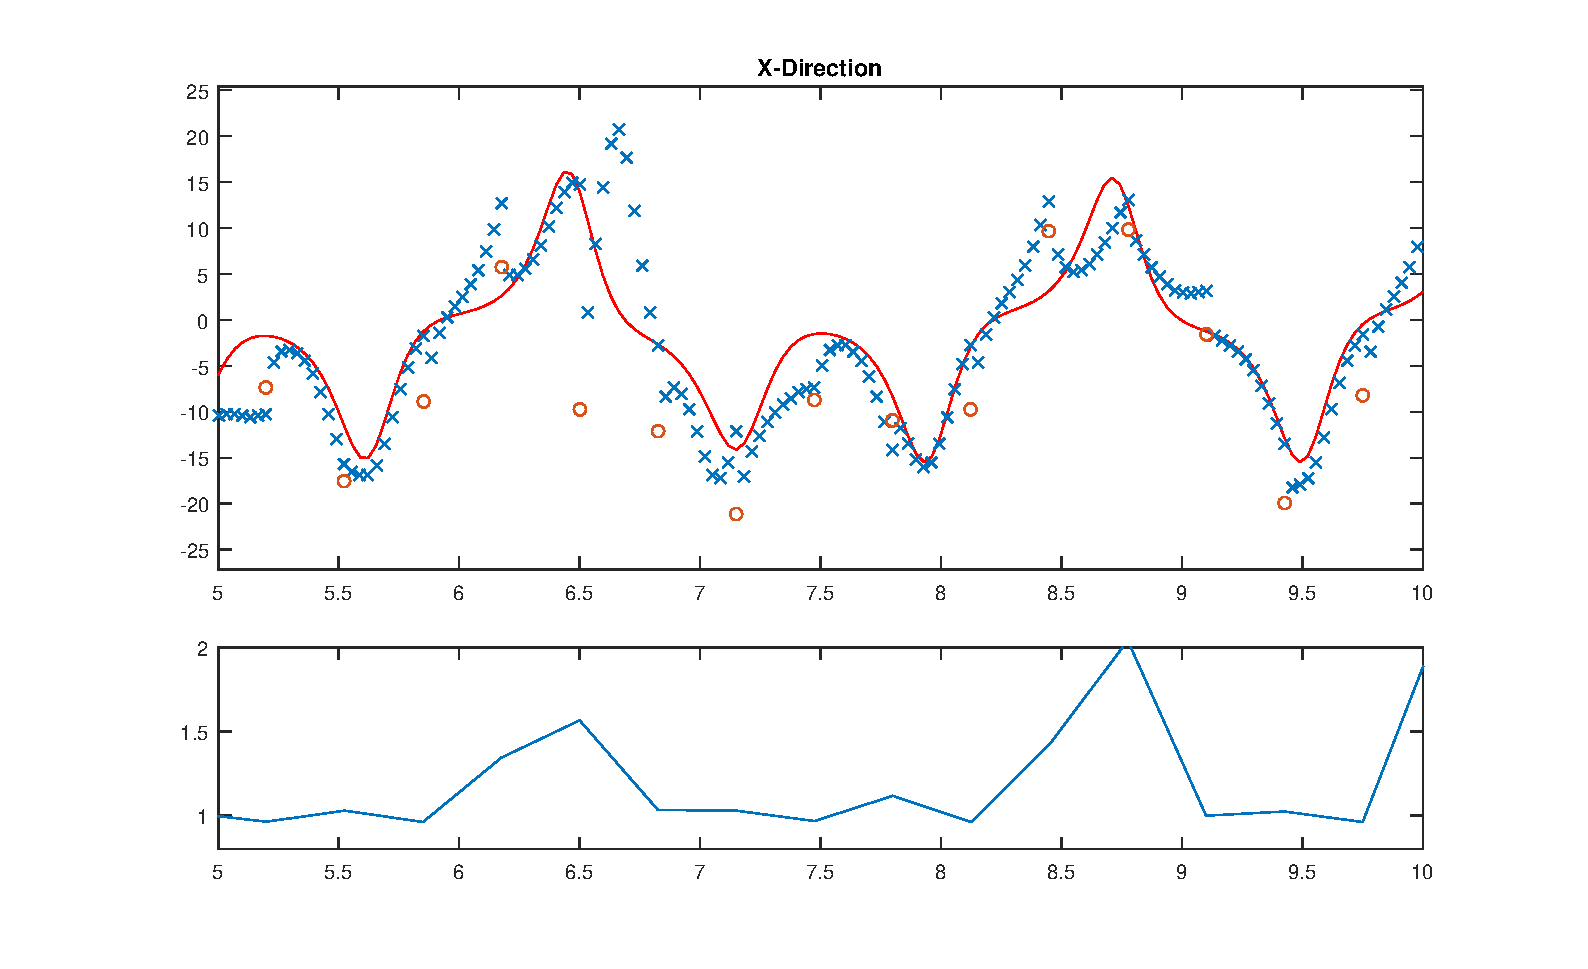
\includegraphics[width=\hsize]{kalman/figures/H2R10S2XP.eps}
\caption{Filteroutput f"ur die X-Achse mit Kovarianzmatrix $P_{11}$ bei direkter Messung mit $H_{1}$ der Zustandsvariablen (oben) und bei indirekter Messung mit $H_{2}$ (unten)}
\label{skript:Kovarianz}
\end{figure}

\section{Beobachtungen und Erkenntnisse}
\rhead{Beobachtungen und Erkenntnisse}
In diesem Kapitel werden aufgestellte Hypothesen besprochen und mit Simulationen verdeutlicht. Das LM63 wird mit den vorgestellten Messmatritzen gemessen und gefiltert. Um die Anzahl Variablen zu reduzieren, wird die folgende dimensionslose Gr"osse verwendet. Ein $F_{R}>1$ bedeutet, dass die Messung genauer ist, als die simulierte Vorhersage, sodass diese st"arker gewichtet wird. Die absolute Fehlervarianz ist f"ur den Filteralgorithmus irrelevant, da lediglich das Verh"altnis Einfluss auf die Gewichtung nimmt.
\[
F_{R}=\frac{Q}{R}
\]
Um den Datenassimilations-Zyklus dimensionslos darzustellen, bildet $S$ die Schrittmenge pro Oszillation. Trotz der chaotischen Oszillation in zwei Richtungen ist diese nahezu konstant. Gilt zum Beispiel $S=2$, so werden pro Oszillation zwei Messungen durchgef"uhrt. Da diese nicht konstant ist, erfolgen die Messungen nicht immer am selben Ort.

Die Untersuchungen werden mit der Oberfl"ache in Abbildung \ref{skript:Oberfl} durchgef"uhrt, wobei  die rote Linie als Realit"at, die blauen Sterne als simulierte Vorhersagen und die roten Kreise als gefilterte Werte dargestellt sind. Sie zeigt auch, das trotz sehr genauer Messung und dadurch einer marginalen Abweichung vom Anfangszustand, eine Vorhersage nur f"ur einen beschr"ankten Zeitraum m"oglich ist. 
\begin{figure}
\centering
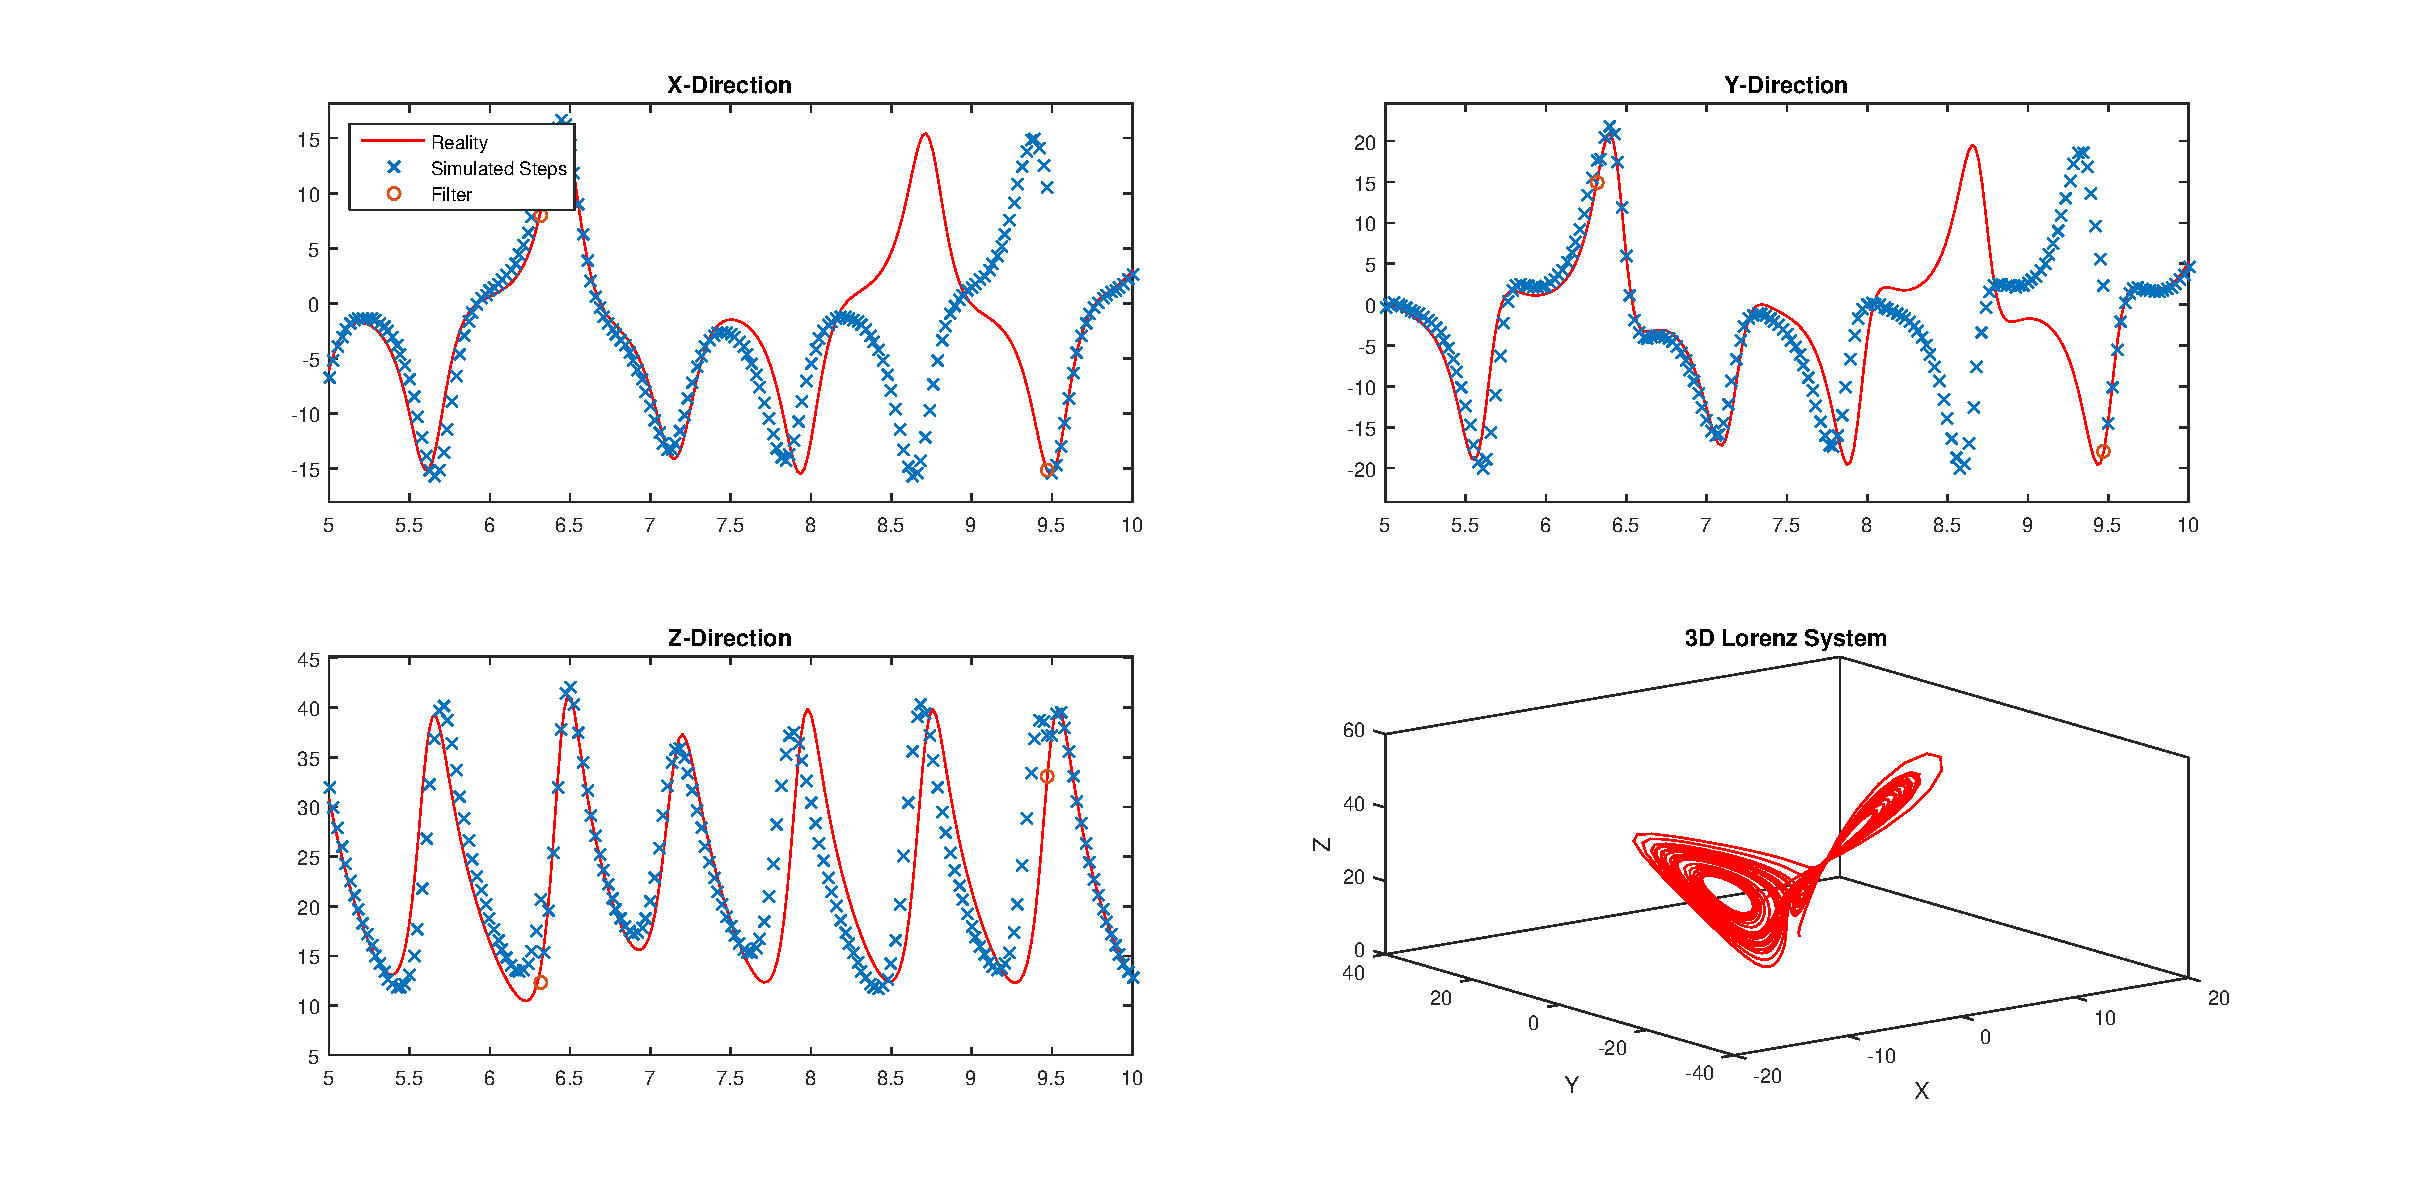
\includegraphics[width=\hsize]{kalman/figures/3dsystemview.eps}
\caption{Arbeitsoberfl"ache mit Legende}
\label{skript:Oberfl}
\end{figure}

\subsection{Vollst"andig erfassbares System}
\rhead{Vollst"andig erfassberes System}
Als vollst"andig erfassbares System gelten hier die Systeme mit den Messmatritzen.
\[H_{1}=\begin{pmatrix}
1 & 0 & 0 \\ 
0 & 1 & 0 \\ 
0 & 0 & 1
\end{pmatrix} 
\text{, }
H_{2}=\begin{pmatrix}
1 & 1 & 0 \\ 
0 & 1 & 1 \\ 
\end{pmatrix}\]
Eine naheliegende Vermutung ist, dass eine genauere Messung, bessere Vorhersagen "uber einen l"angeren Zeitraum erlaubt. Also aus einem gr"osseren $F$ resultieren besser Vorhersagen, was die oberen beiden Bilder in Abbildung \ref{skript:H1S1} illustrieren. Dies gilt aber nur, wenn das Systemmodell gut mit der Realit"at korreliert, was in diesem Versuch der Fall ist, da die Realit"at genau dem Systemmodell entspricht.
Was ein Vergleich der unteren Bilder deutlich zeigt, ist dass der Mehraufwand an Messgenauigkeit auch dadurch kompensiert werden kann, in dem zu einem g"unstigerem Zeitpunkt gemessen wird. Hierbei zeigt sich deutlich das Chaos des System, wo nicht quantitativ beurteilt werden kann, zu welchen Zeitpunkt welche Genauigkeiten notwendig sind.
\begin{figure}
\centering
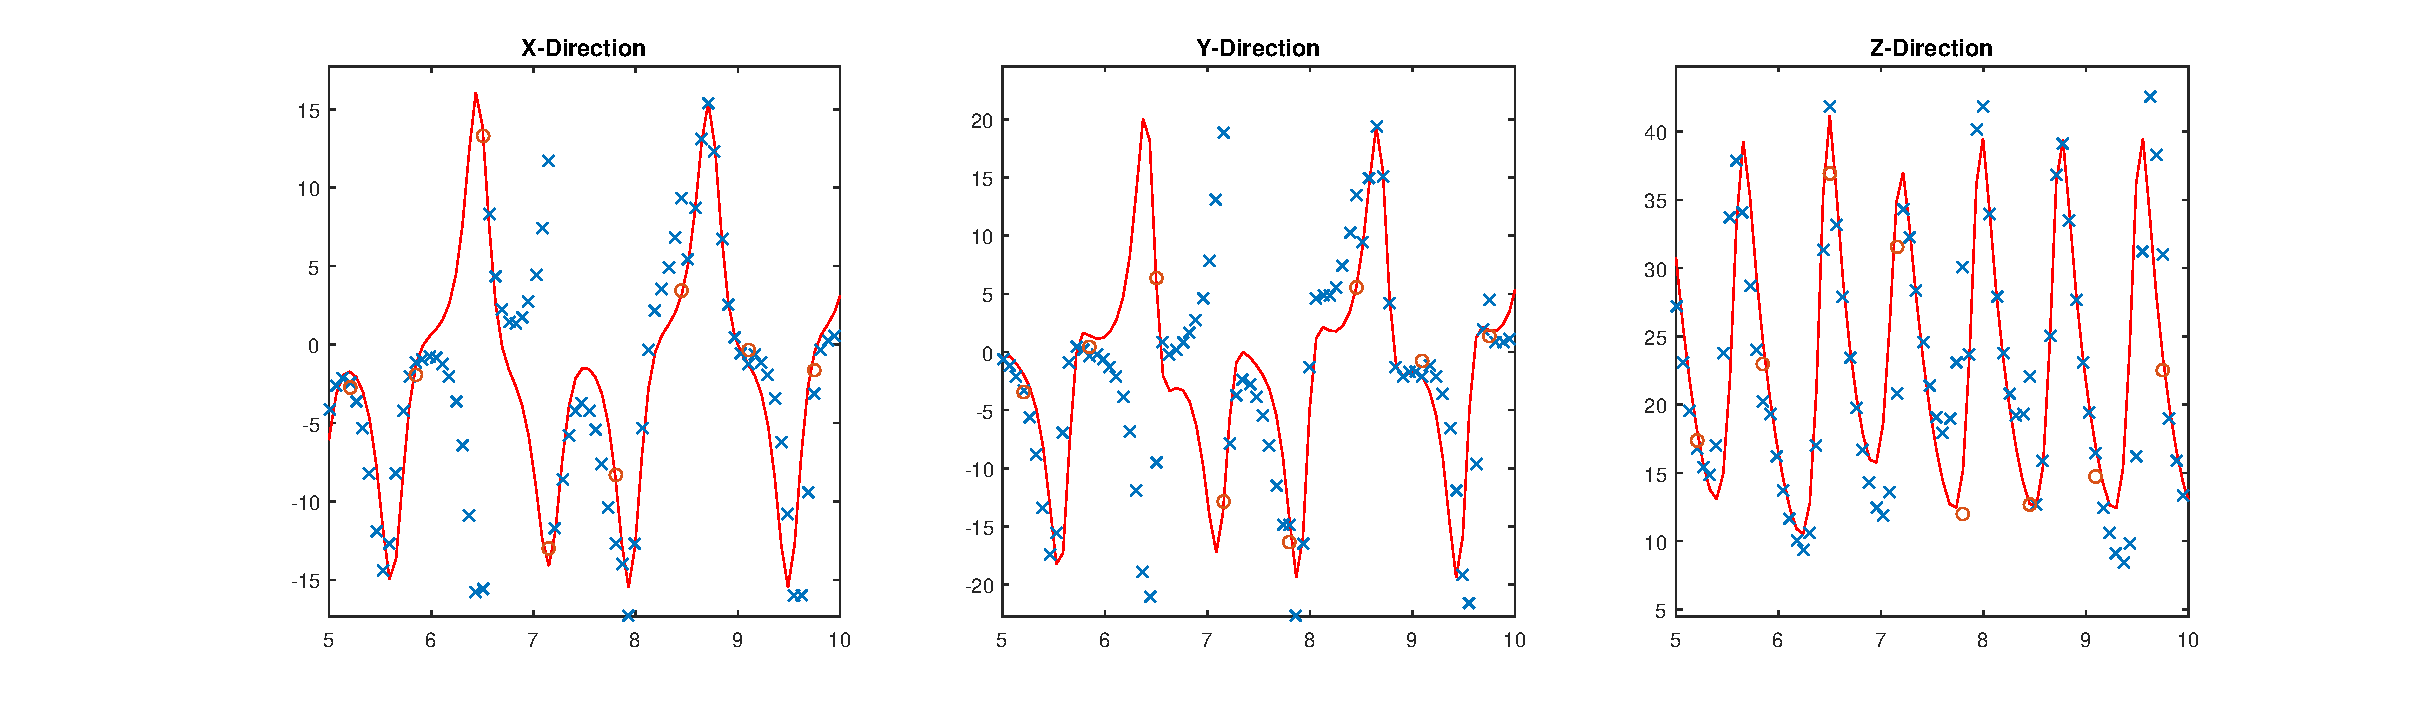
\includegraphics[width=\hsize]{kalman/figures/H1R10S1.eps}
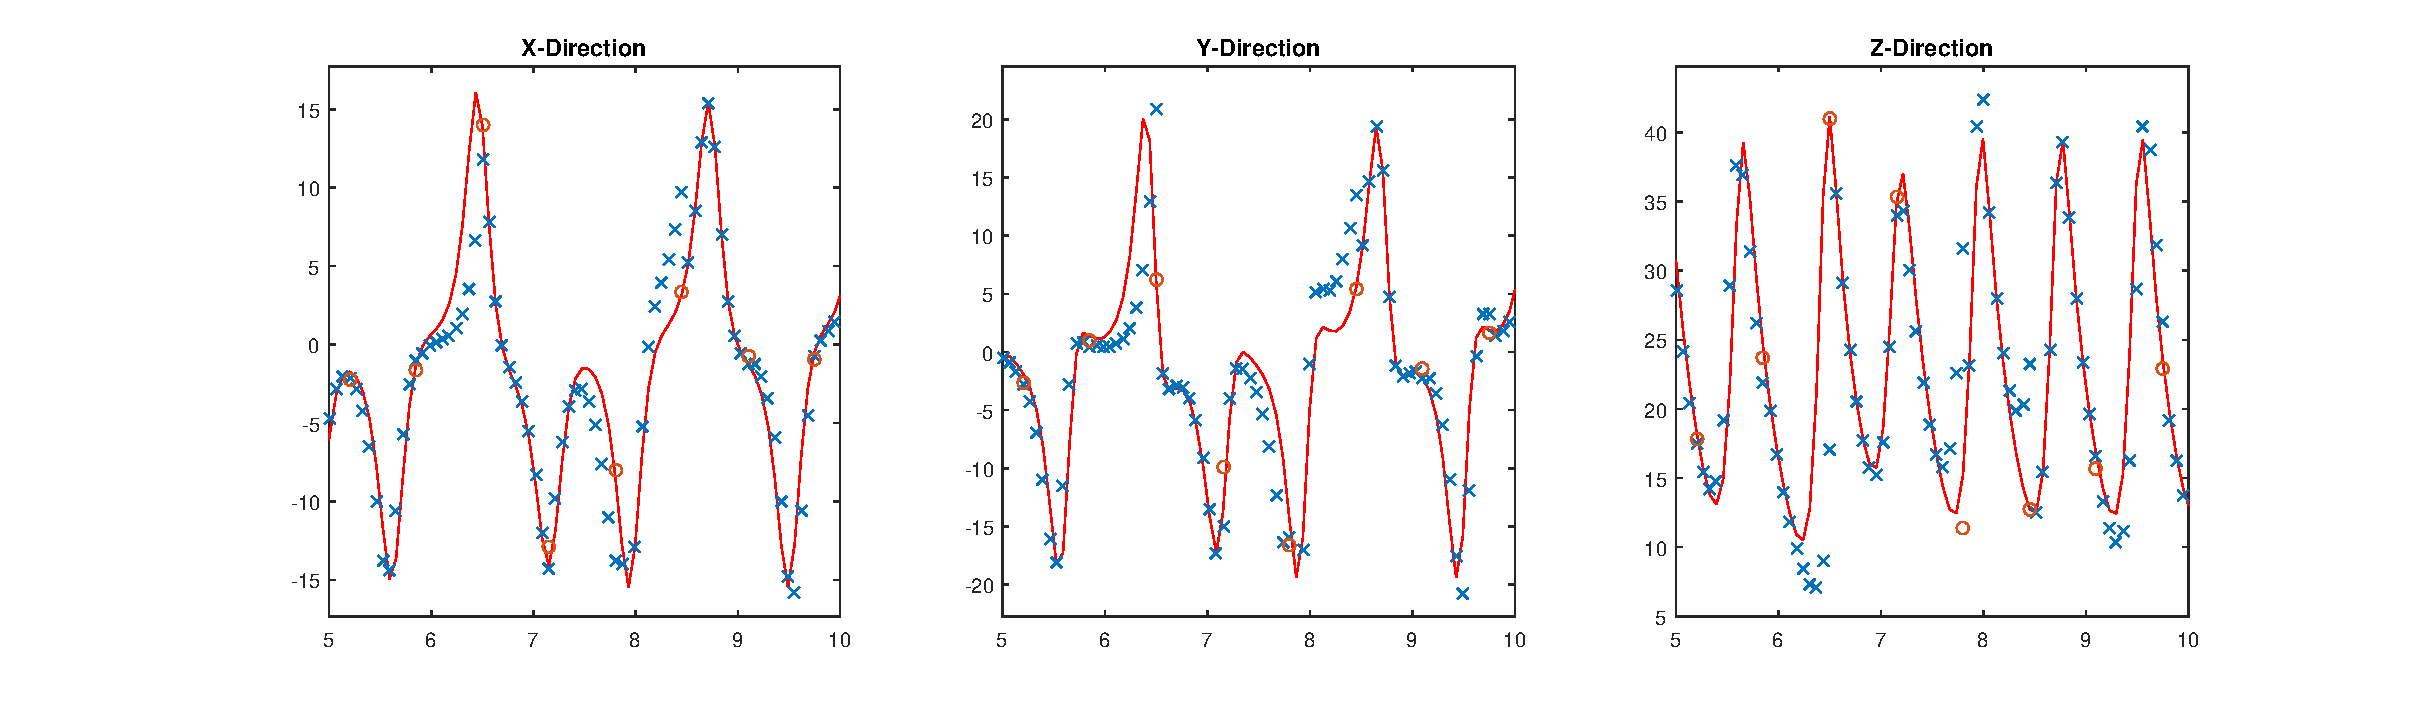
\includegraphics[width=\hsize]{kalman/figures/H1R20S1.eps}
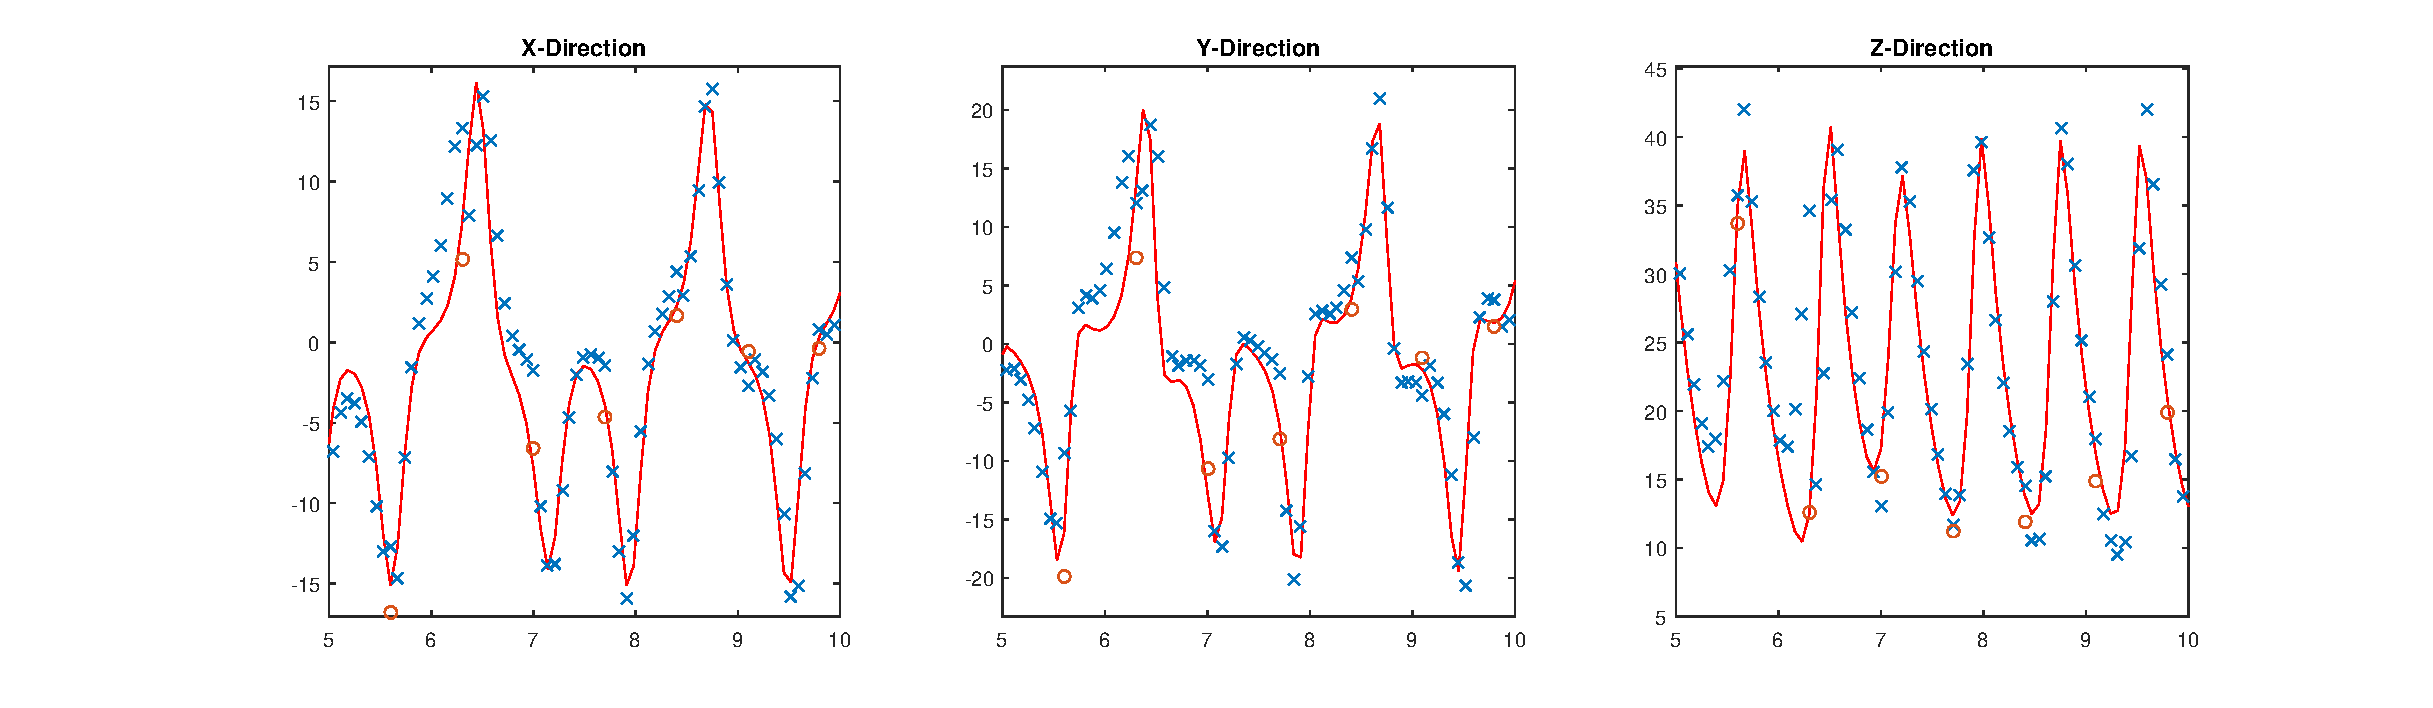
\includegraphics[width=\hsize]{kalman/figures/H1R10S1aS.eps}
\caption{Messmatrix H1 jeweils mit S=1 und F=10 (oben), F=20 (mitte) und F=10 (unten), letztere mit versetzter Messung}
\label{skript:H1S1}
\end{figure}

Abbildung \ref{skript:H1S2} zeigt das Modell in dem Messungen zweimal pro Oszillation zur Verf"ugung stehen. So steht eine korrigierende Messung schneller zur Verf"ugung, jedoch wird auch der Vorhersage-Zeitraum k"urzer, was denn Zweck des Filters zunehmend einschr"ankt. Deutliche Verbesserungen gegen"uber vorhin sind nicht zu erkennen, sie werden in diesem Beispiel sogar schlechter. Je h"aufiger das gemessen wird, desto weniger relevant wird zudem der Zeitpunkt der Messung.
Um die Relevanz nochmals zu verdeutlichen, eine Vorhersage in die entgegengesetzte Richtung bedeutet, dass die Drehrichtung  der Konvektionsstr"ome falsch gesch"atzt wurde.
\begin{figure}
\centering
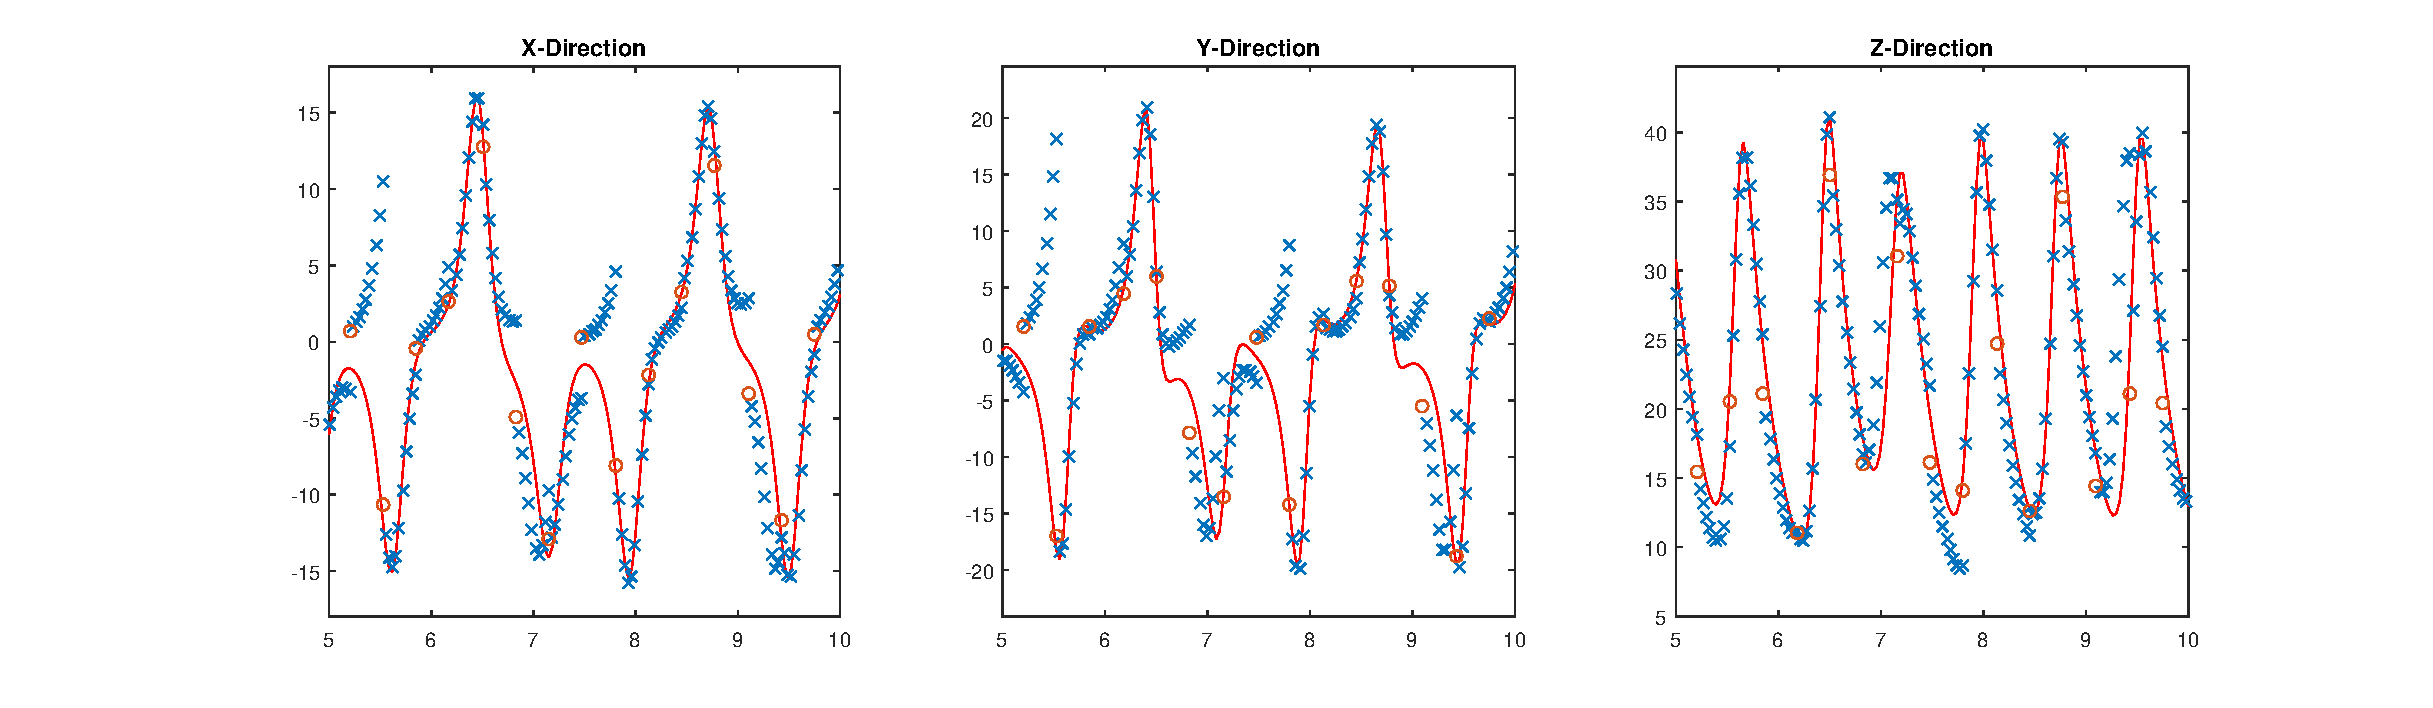
\includegraphics[width=\hsize]{kalman/figures/H1R10S2.eps}
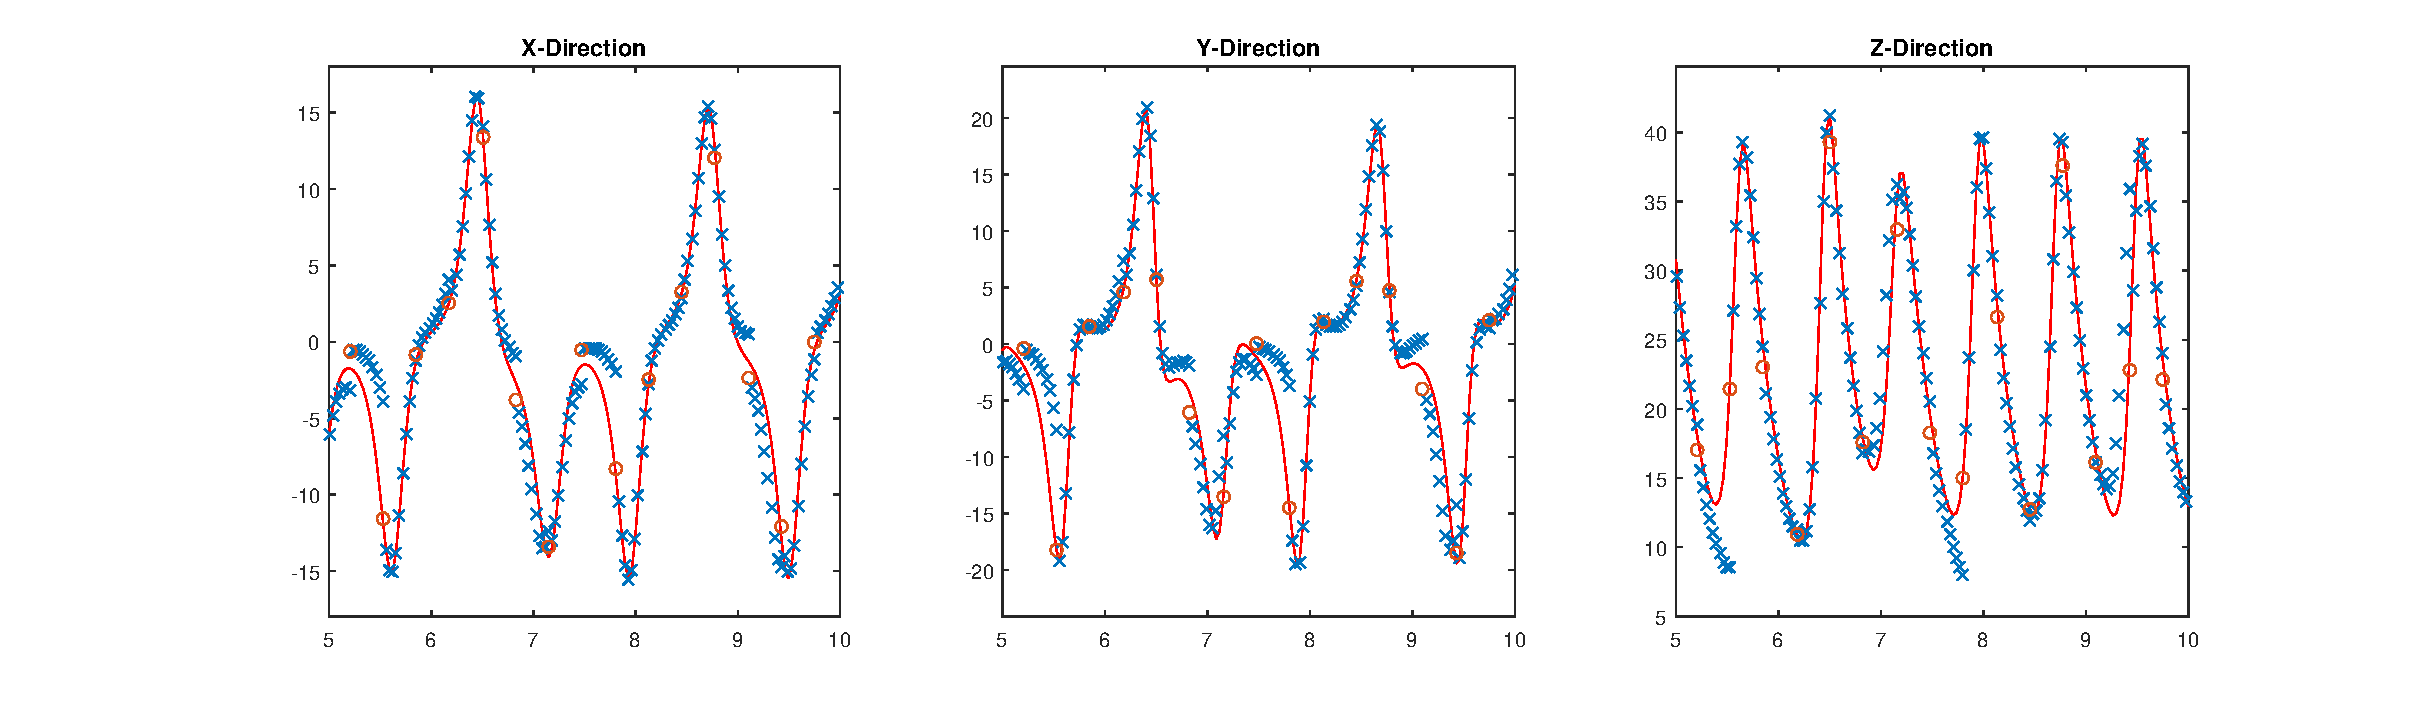
\includegraphics[width=\hsize]{kalman/figures/H1R25S2.eps}
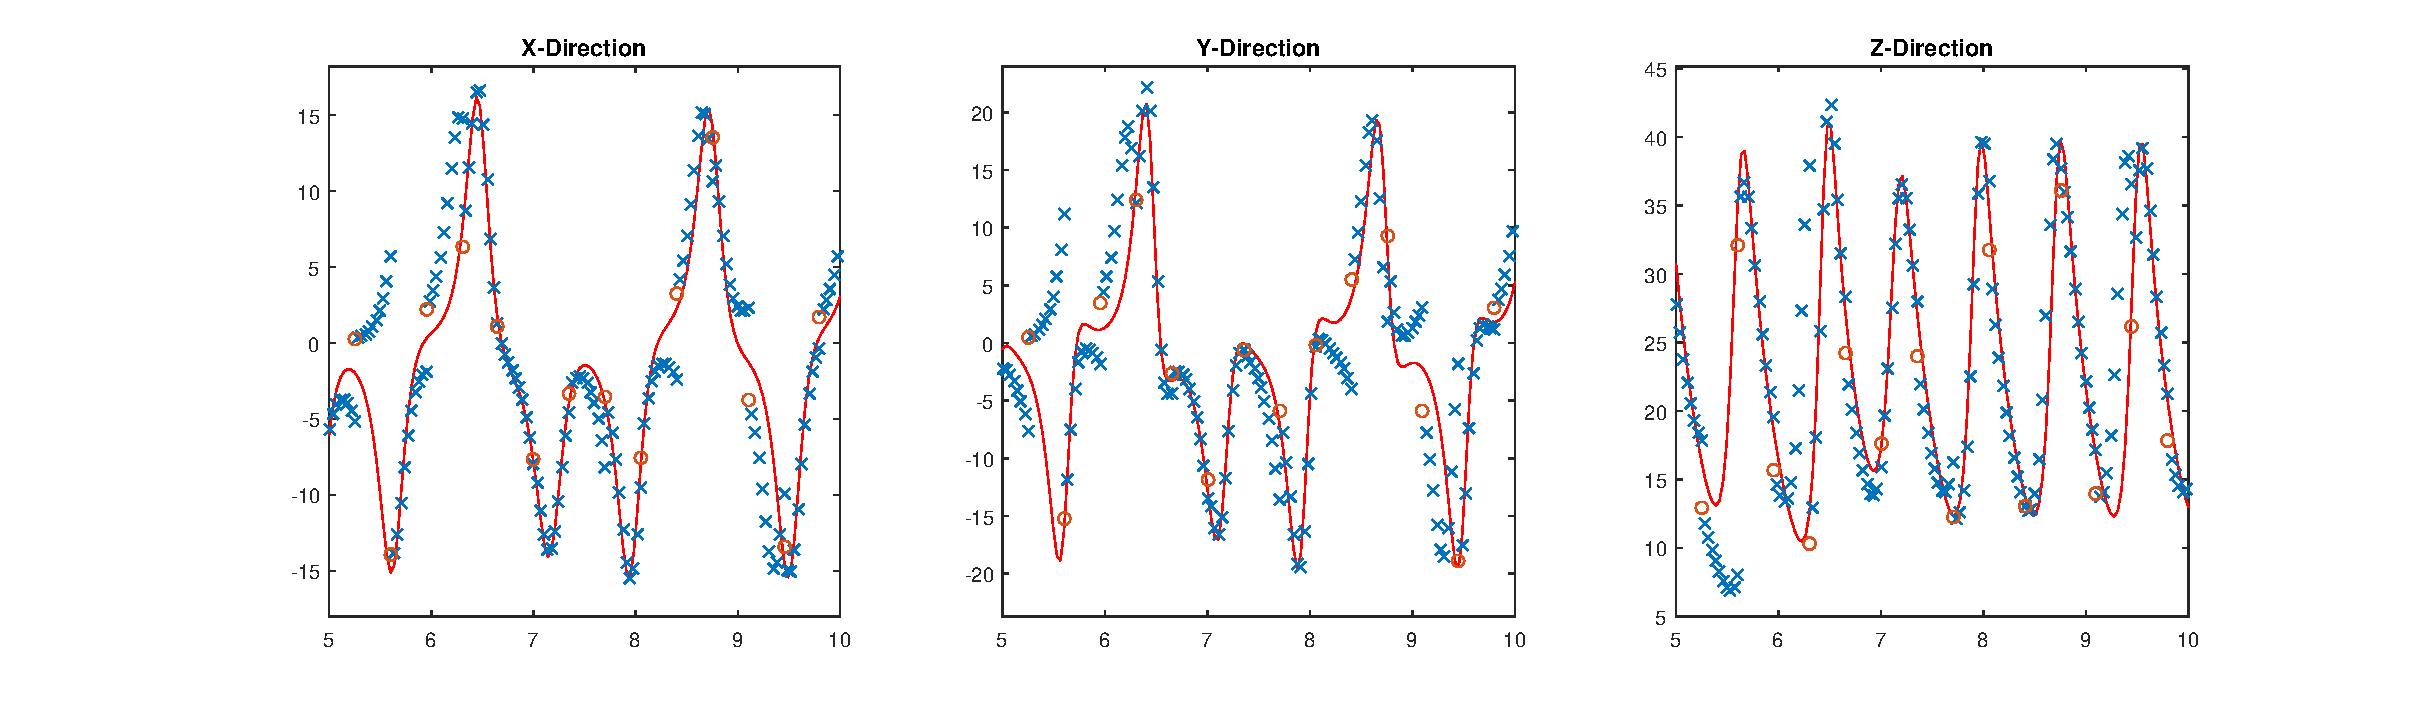
\includegraphics[width=\hsize]{kalman/figures/H1R10S2aS.eps}
\caption{Messmatrix H1 jeweils mit S=2 und F=10 (oben), F=25 (mitte) und F=10 (unten), letztere mit versetzter Messung}
\label{skript:H1S2}
\end{figure}

Bei f"unf Messungen pro Oszillation (Abbildung \ref{skript:H1S5}), trotz niedriger Messgenauigkeit, ist eine exakte Rekonstruktion der simulierten Realit"at m"oglich. Simulierte Zwischenschritte sind meist korrekt, sind aber nur f"ur kurze Intervalle verf"ugbar und damit immer weniger interessant.
\begin{figure}
\centering
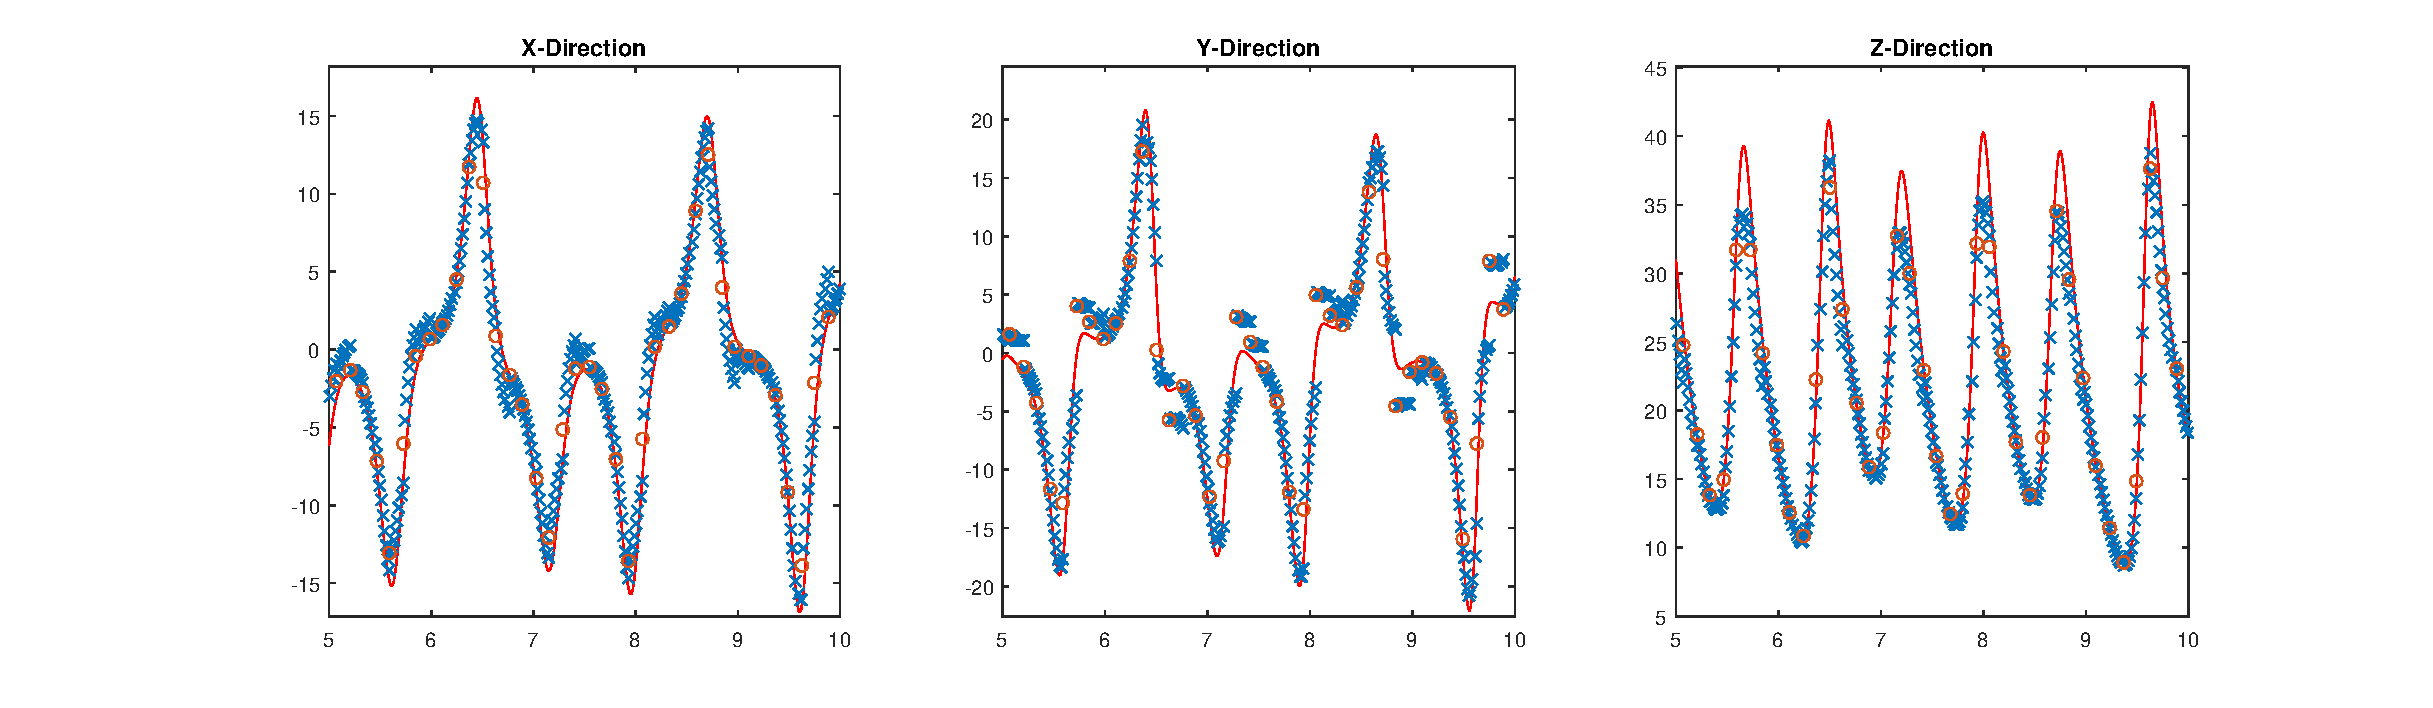
\includegraphics[width=\hsize]{kalman/figures/H1R05S5.eps}
\caption{Messmatrix H1 mit S=5 und F=5}
\label{skript:H1S5}
\end{figure}

K"onnen alle Messwerte gemessen werden, aber nur als Linearkombination wie mit H2, sind Verschleppungen von Oszillationen aus einer Achse in eine andere erkennbar. In Abbildung \ref{skript:H2S1} ist zu erkennen, das trotz dieser Schwierigkeit, der Filter die Realit"at sehr gut vorhersagen kann. Jedoch scheint eine Verbesserung der Messgenauigkeit keine Verbesserung der Vorhersagen zu bewirken.
Auch die Messrate zu verdoppeln l"ost die Problematik nur bedingt, da nun h"ufiger kombinierte Werte gemessen werden, die um den Wert anderer Koordinaten verschoben sind. Die Simulation ist hier verl"asslicher als mit der Messmatrix H1, trotzdem ist eine regelm"assige Referenzierung unterl"asslich. So verlief der Versuch unter allen bisher genannten Bedingungen negativ, den Fehler der Simulation st"rker zu gewichten als den Messfehler.

\begin{figure}
\centering
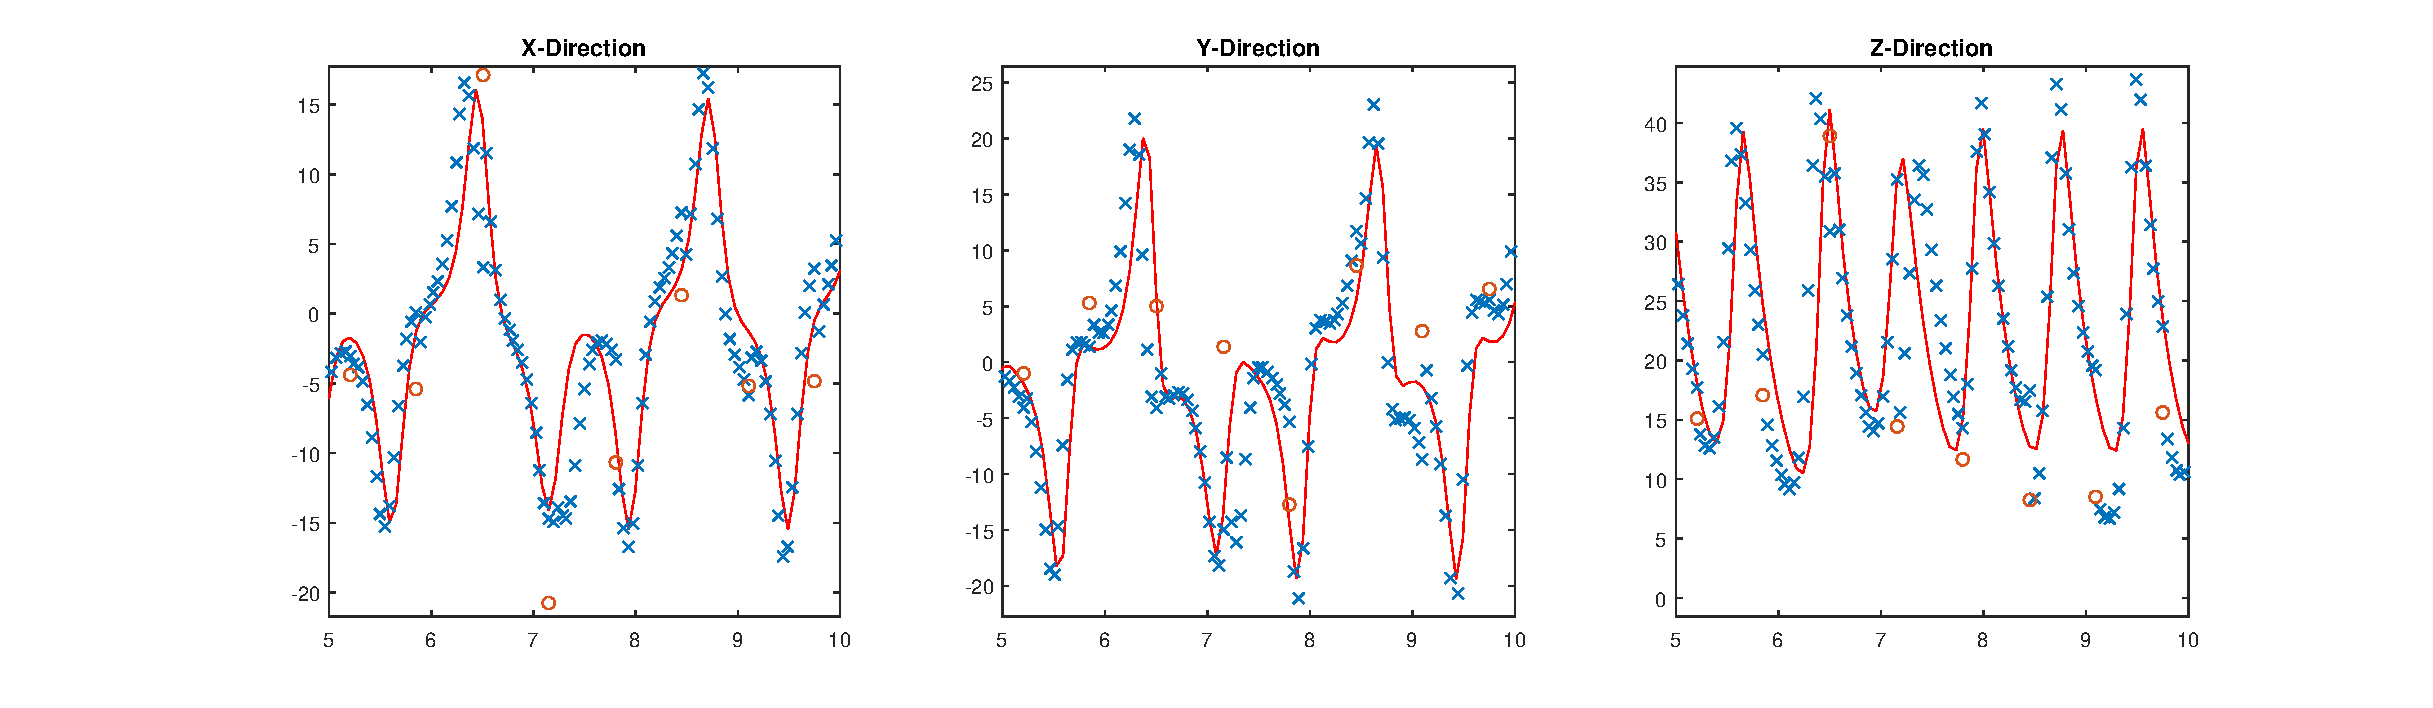
\includegraphics[width=\hsize]{kalman/figures/H2R05S1.eps}
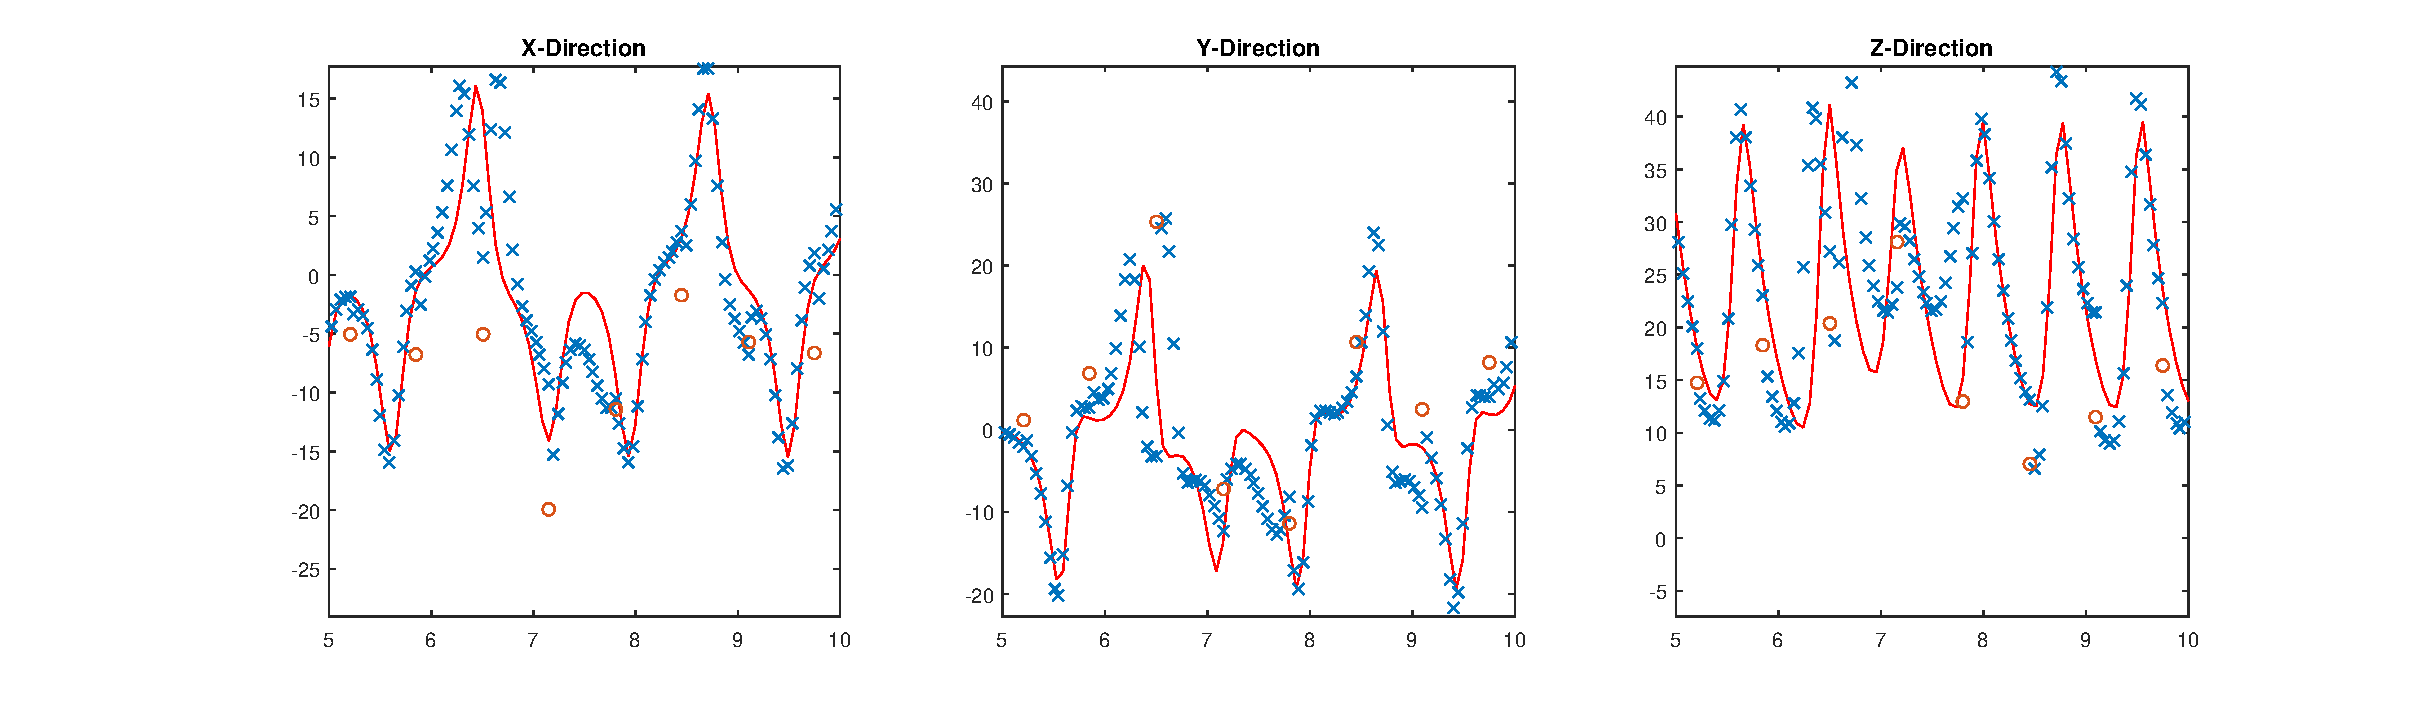
\includegraphics[width=\hsize]{kalman/figures/H2R20S1.eps}
\caption{Messmatrix H2 mit S=1 und F=5 (oben) und F=20 (unten)}
\label{skript:H2S1}
\end{figure}

\begin{figure}
\centering
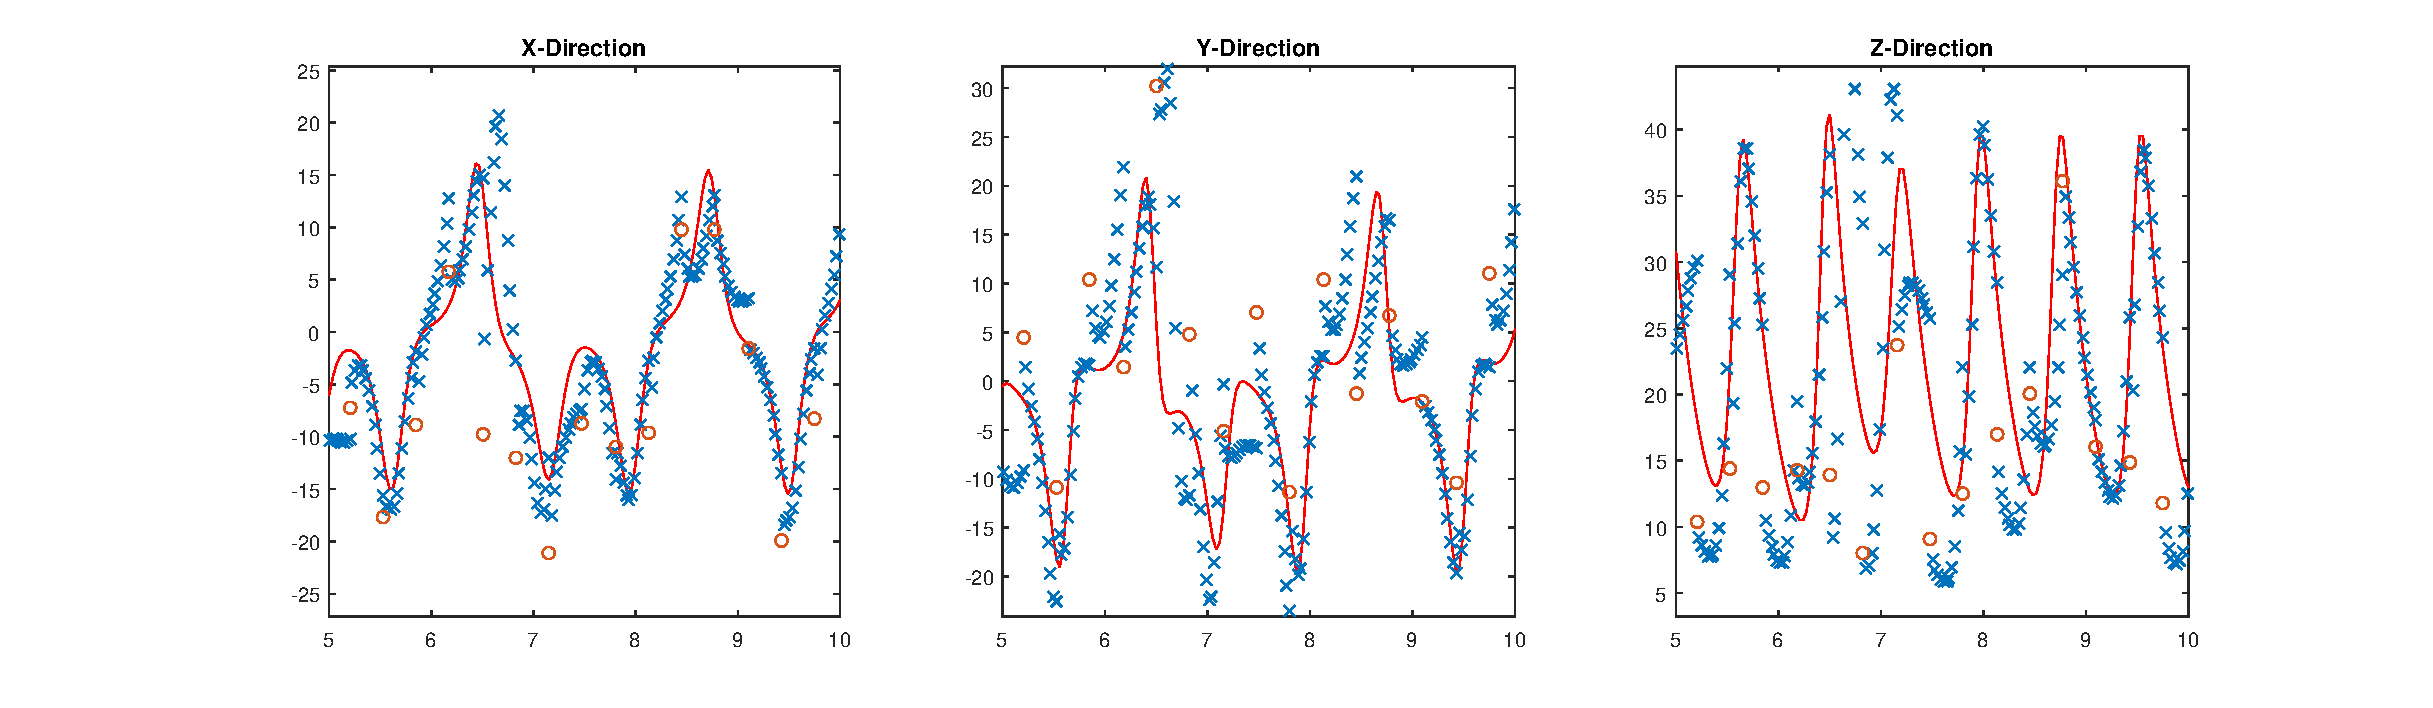
\includegraphics[width=\hsize]{kalman/figures/H2R10S2.eps}
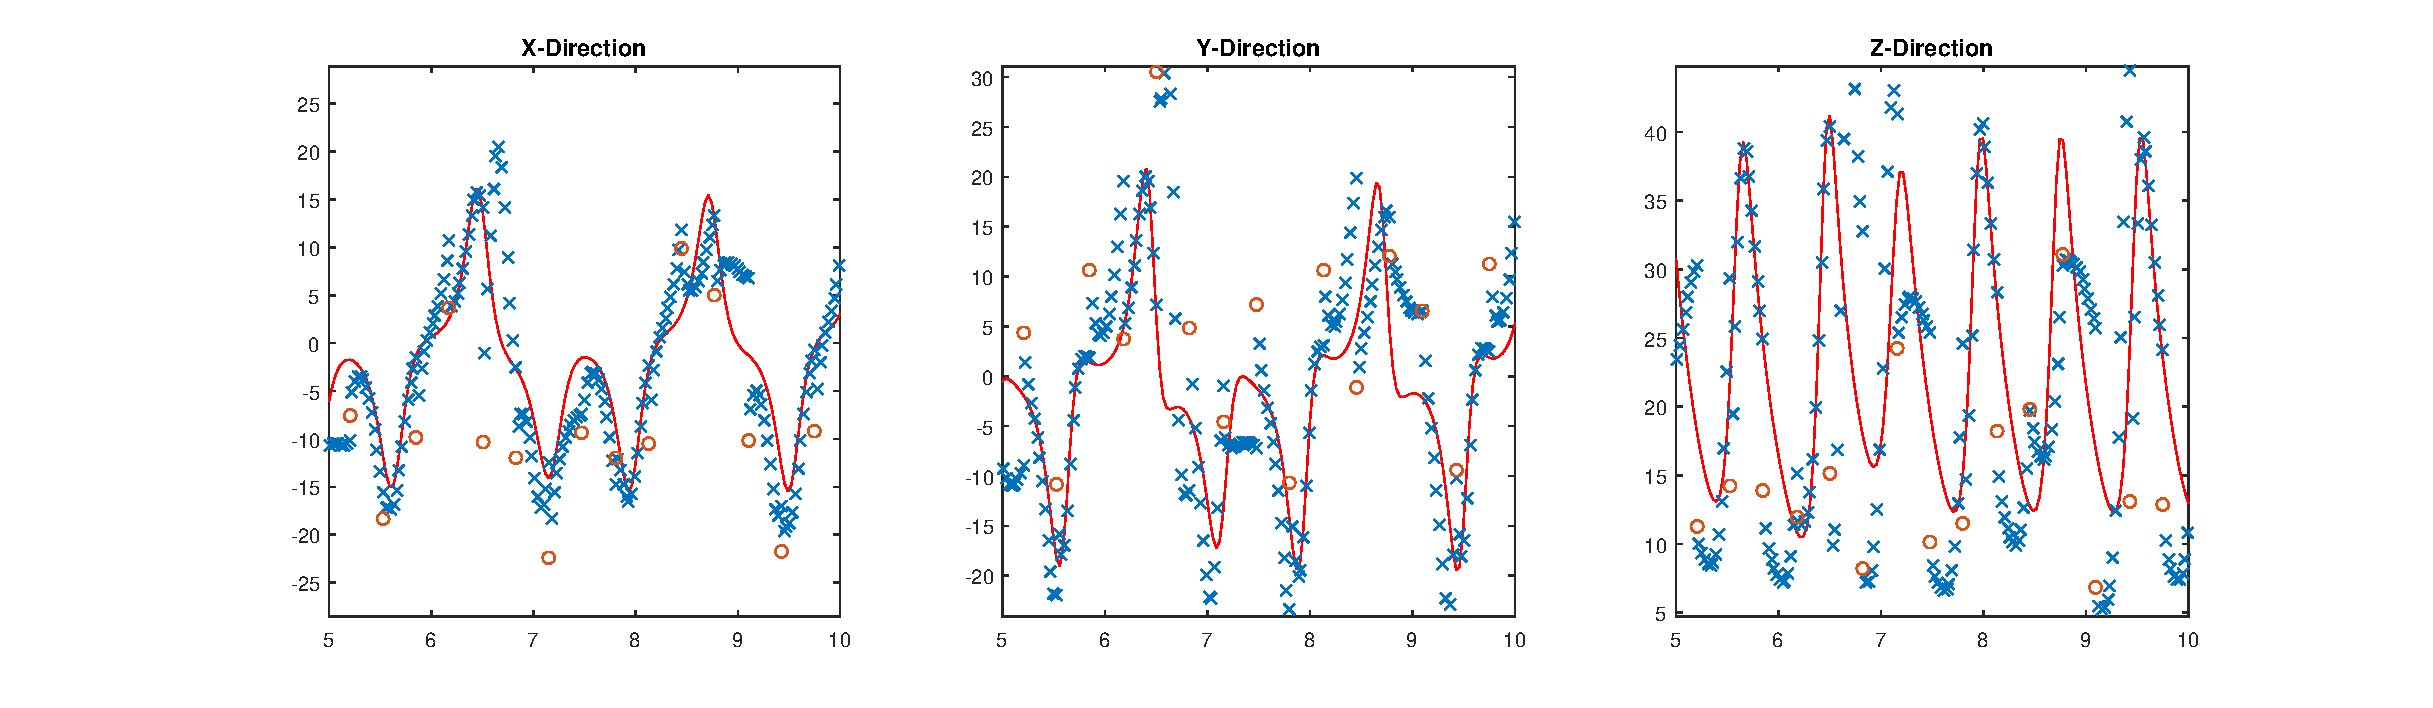
\includegraphics[width=\hsize]{kalman/figures/H2R20S2.eps}
\caption{Messmatrix H2 mit S=2 und F=10 (oben) und F=20 (unten)}
\label{skript:H2S2}
\end{figure}

Wird die Messkadenz noch einmal wie in Abbildung \ref{skript:H2S5} erh"oht, scheinen einzig die Werte in X und Z Richtung verl"asslichere Vorhersagen und bessere gefilterte Daten zu liefern. Der Y-Wert und deren Simulationen zeigen h"aufig gar in die falsche Richtung. Dies ist kann darauf zur"ck zu f"uhren, da in der Gleichung f"ur Y alle drei Koordinaten Einfluss nehmen und so eine Messung  schwierig ist. Aufgrund der resultierenden Abweichung folgt dann eine schlechte Vorhersage des Systems.

\begin{figure}
\centering
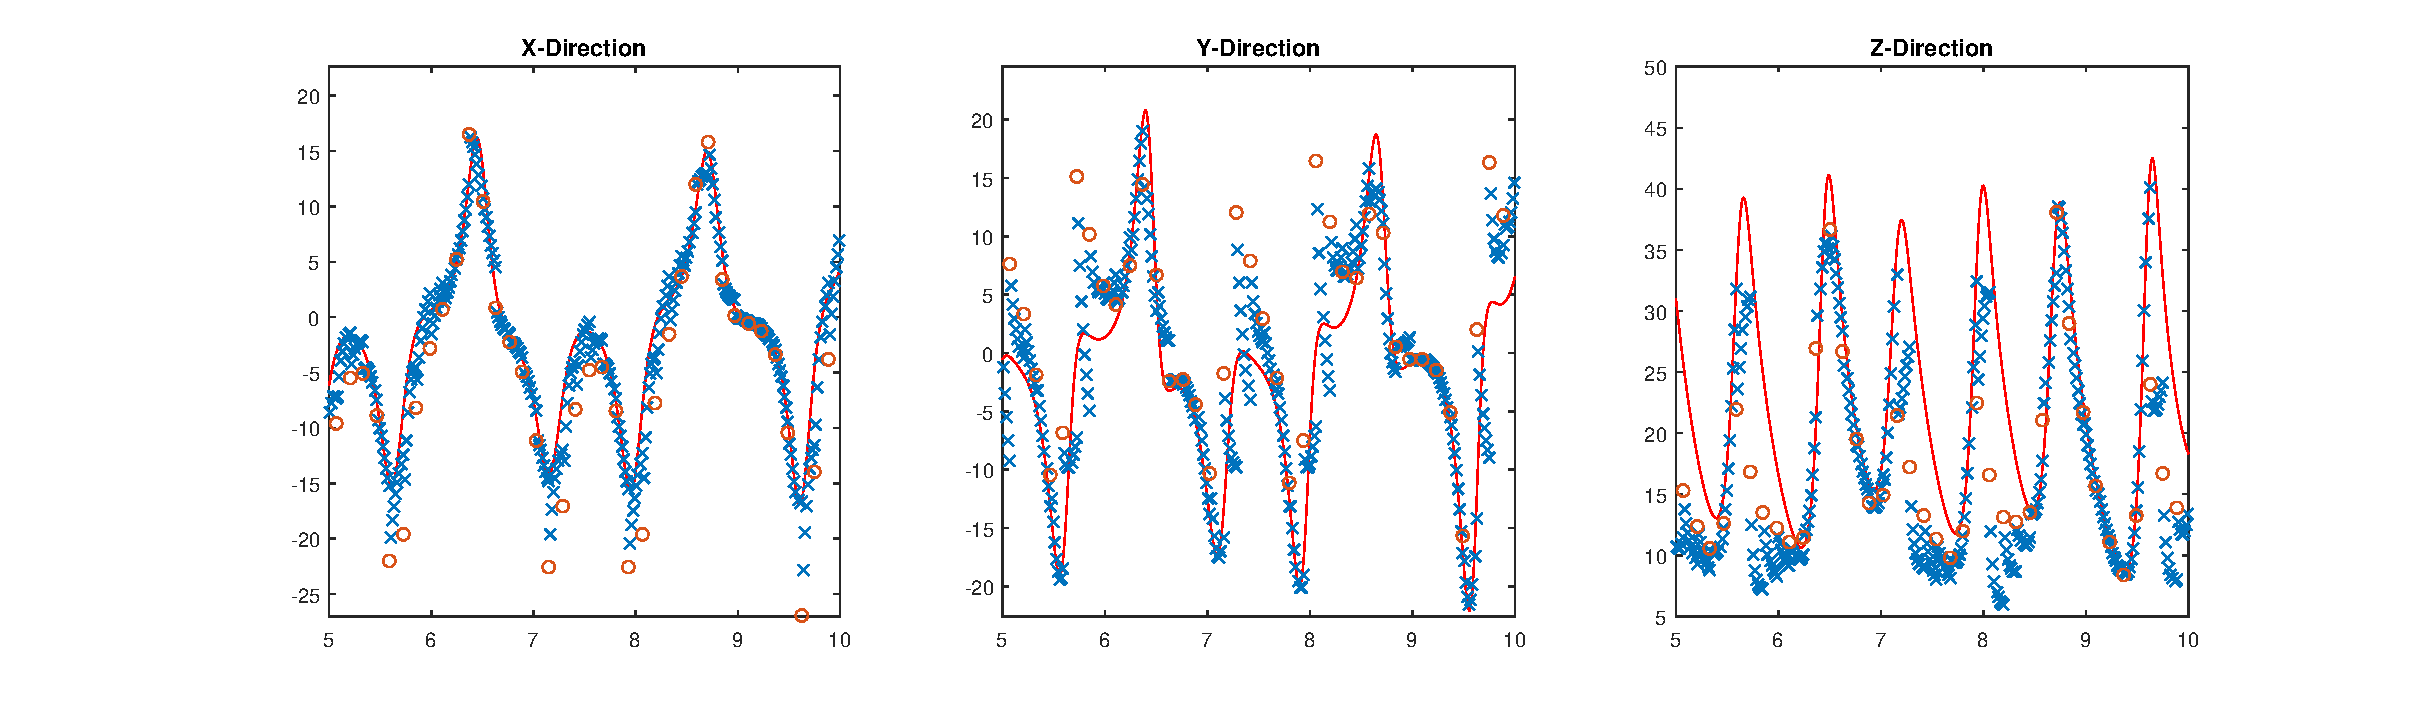
\includegraphics[width=\hsize]{kalman/figures/H2R05S5.eps}
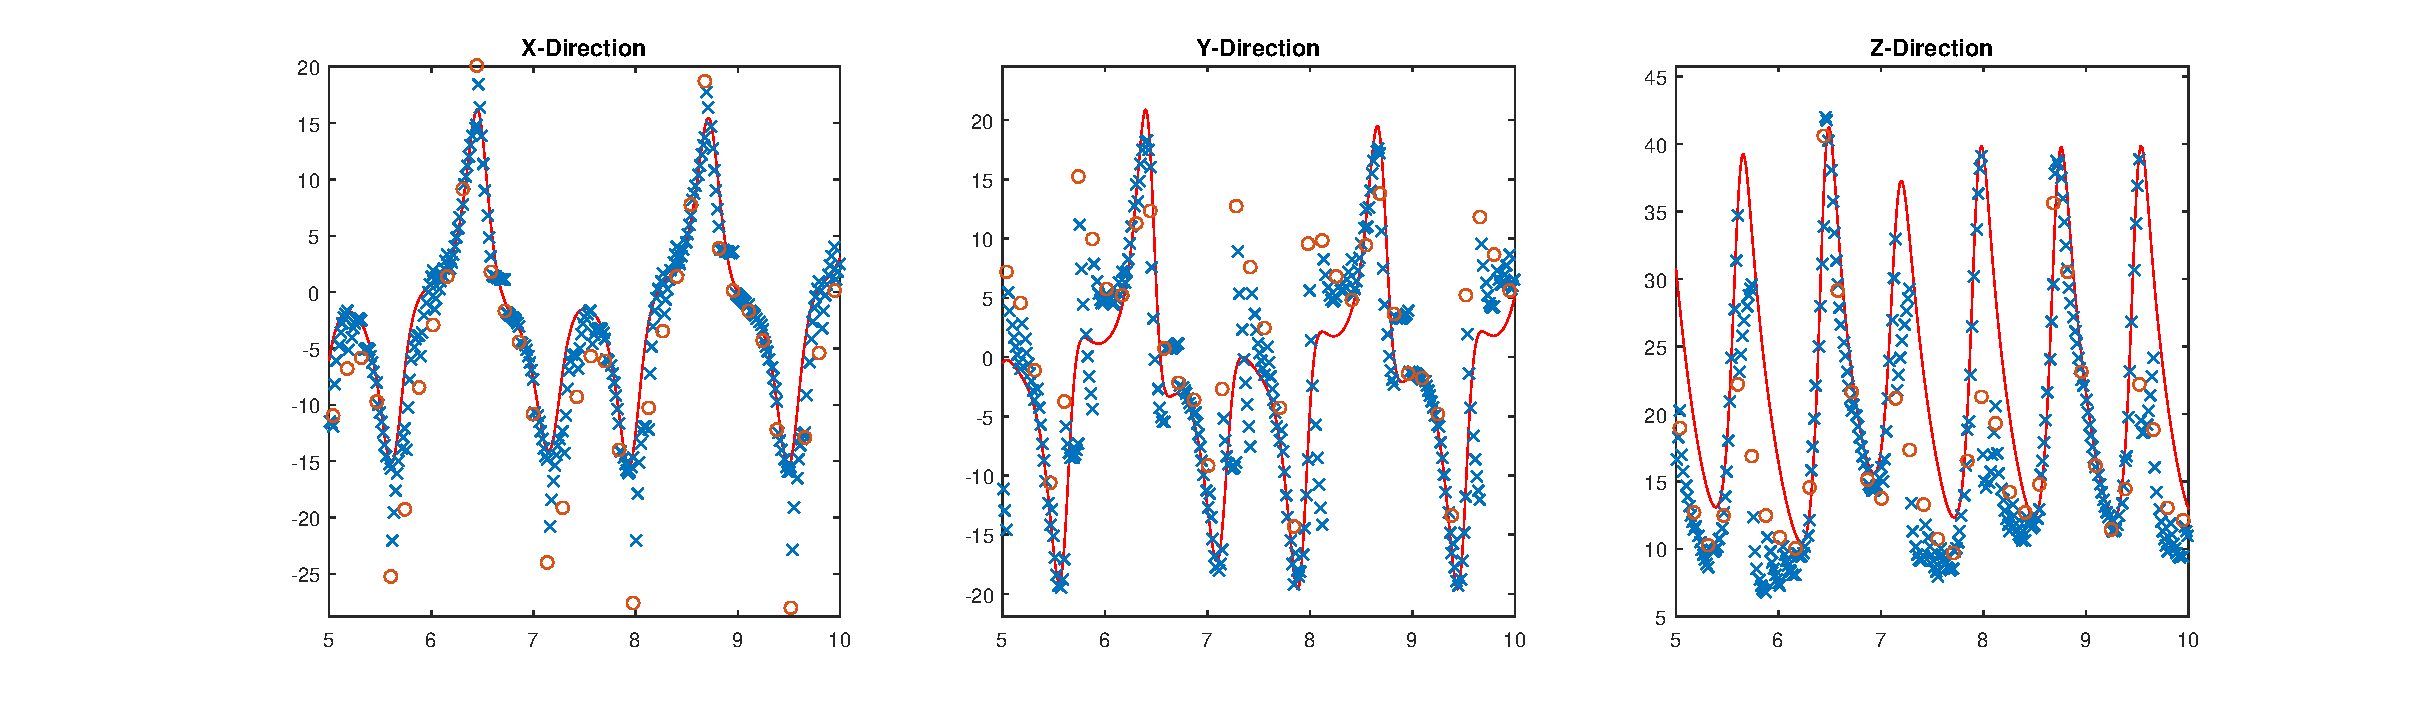
\includegraphics[width=\hsize]{kalman/figures/H2R10S5.eps}
\caption{Messmatrix H2 mit S=5 und F=5 (oben) und F=10 (unten)}
\label{skript:H2S5}
\end{figure}

\subsection{Unvollst"andig erfassbares System}
\rhead{Unvollst"andig erfassberes System}
Nun noch die unvollst"andig erfassbaren Systeme mit den Messmatritzen $H3$ und $H4$.
\[H_{3}=\begin{pmatrix}
1 & 0 & 0 \\ 
0 & 1 & 0 \\ 
\end{pmatrix} 
\text{, }
H_{4}=\begin{pmatrix}
1 & 0 & 0 \\ 
0 & 0 & 1
\end{pmatrix}\]

Gem"ass der rechten Seite des Lorenz Modells ist bekannt, dass alle drei Werte von einander abh"angen, und so folglich alle zur Verf"ugung stehen m"ussten. In Abbildung \ref{skript:H3} der Versuch, mit verschiedenen $F$ und $S$ der Situation trotzdem Herr zu werden. Erst im mittleren Bild mit $S=2$ und $F=20$ ist die Anzahl der richtig vorhergesagten Werten,abgesehen von den Werten f"ur Z, in der "Uberzahl. Wird die Messkadenz weiter erh"oht, folgen die Simulation gut der Realit"at, wobei die Schwierigkeit erneut bei den Werten f"ur Y liegt, da Z Werte komplett auf Simulationen beruhen. Das "uberhaupt eine Rekonstruktion m"oglich ist, ist der Tatsache geschuldet, dass die Z-Achse keine Informationen "uber das Chaos des Systems enth"alt, daher ob die Konvektionszelle mit oder gegen den Uhrzeigersinn str"omt. Dies ist sowohl in den diversen Z-Ansichten zu erkennen, wo die Werte mit ann"ahernd gleichbleibender Oszillation und Amplitude vorkommen, sowie in der Abbildung \ref{skript:zview} mit der Sicht in die XY-Ebene.
Folglich kann mit einer h"oheren Messkadenz bessere Ergebnisse erzielt werden, als wenn die Messgenauigkeit erh"oht wird.

\begin{figure}
\centering
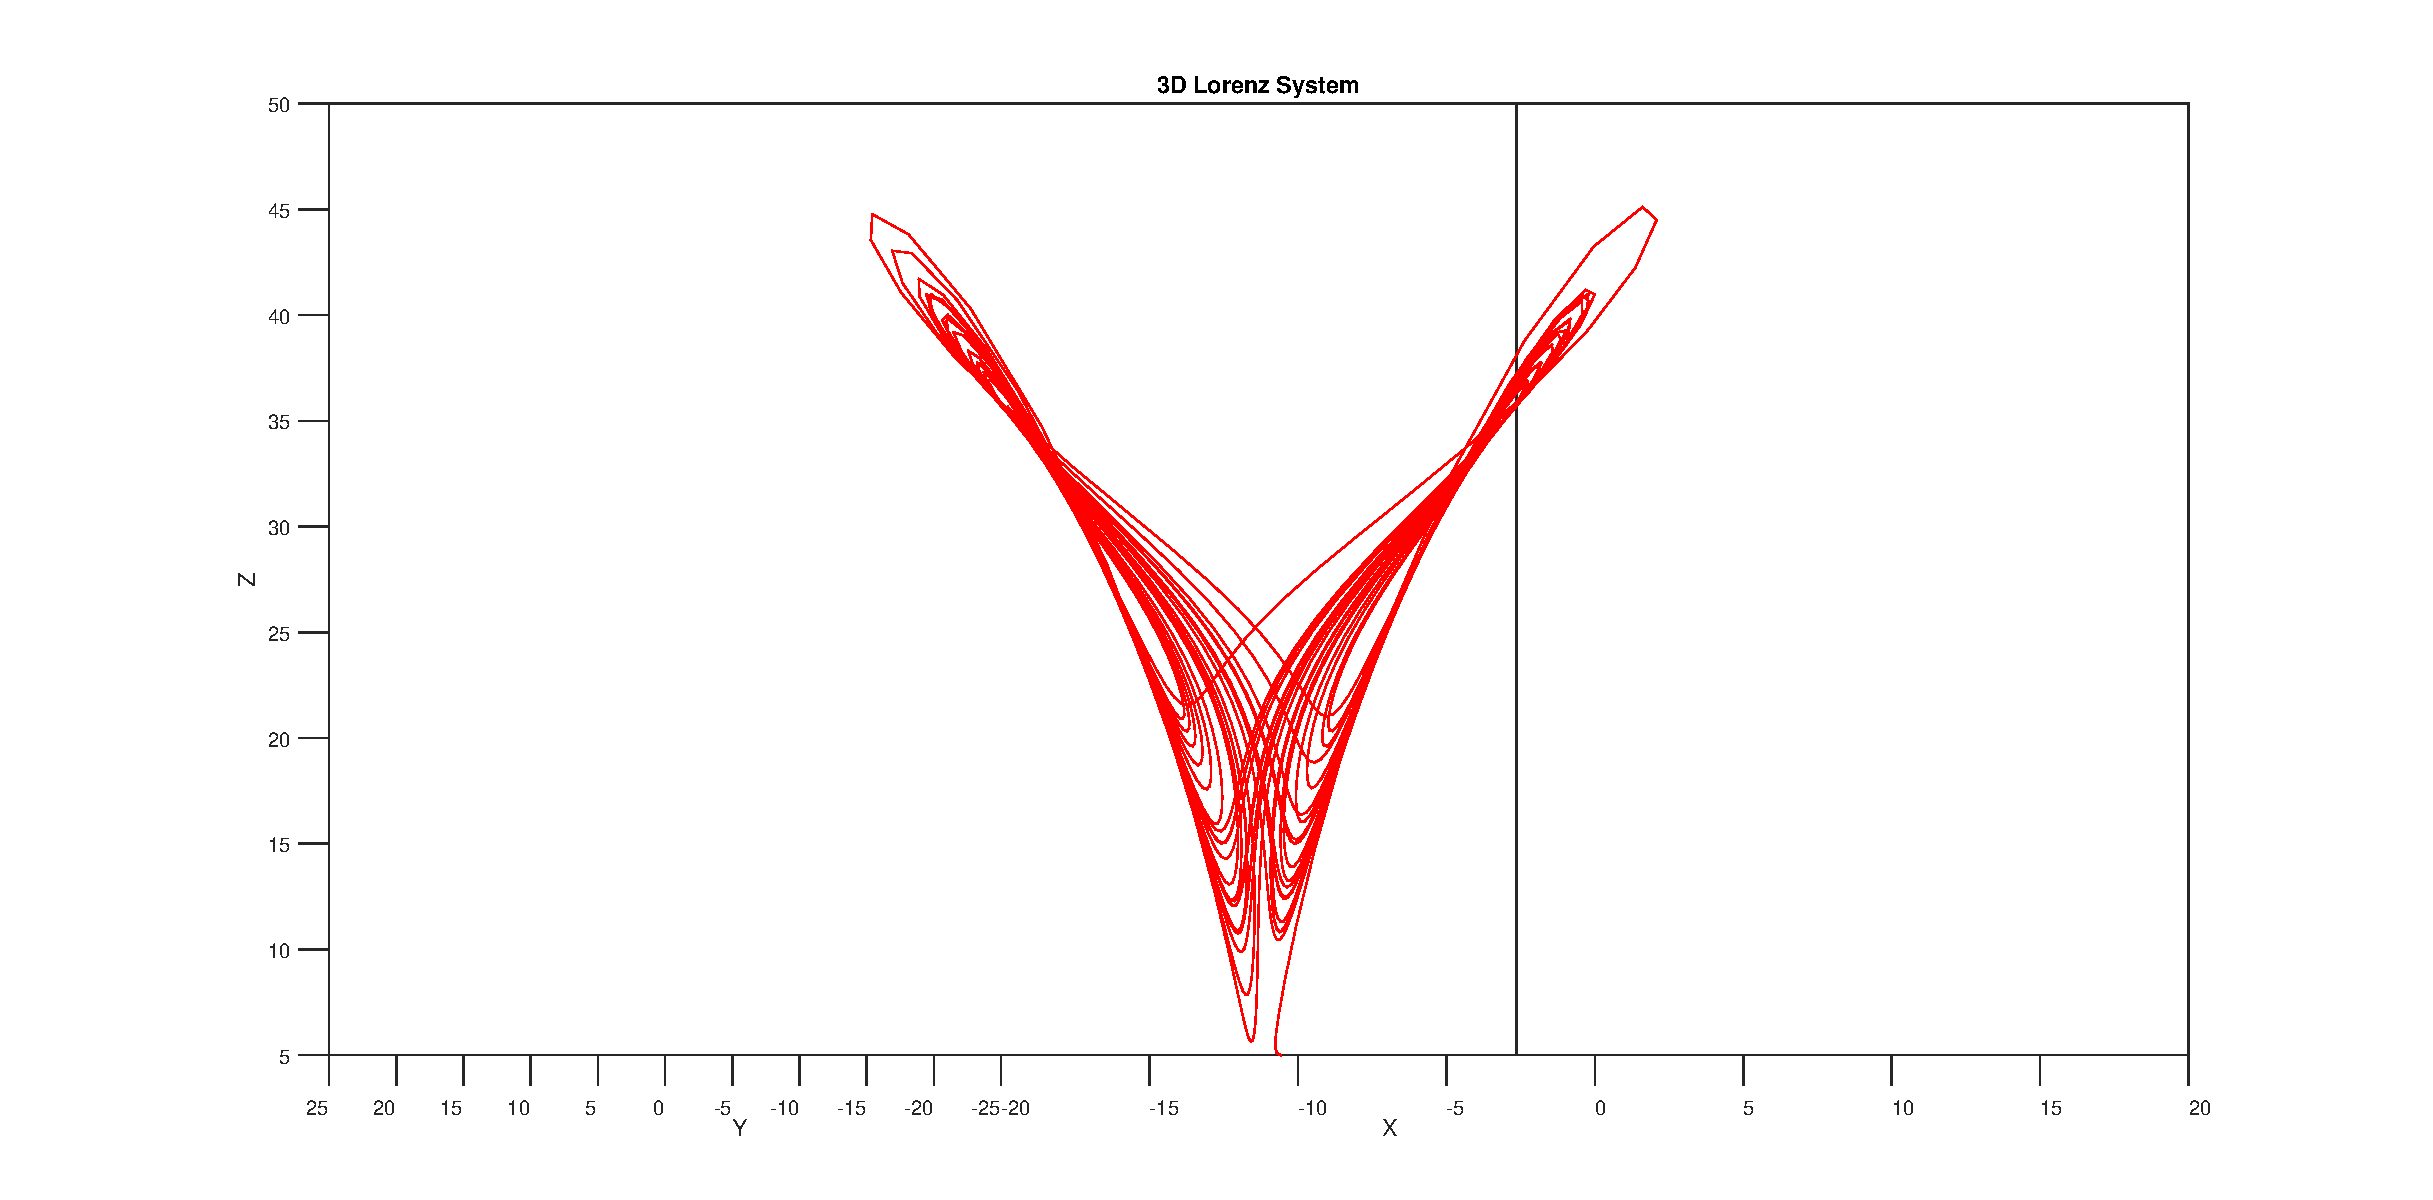
\includegraphics[width=\hsize]{kalman/figures/zview.eps}
\caption{3-D Lorenz System mit Sicht auf Z-Achse}
\label{skript:zview}
\end{figure}

\begin{figure}
\centering
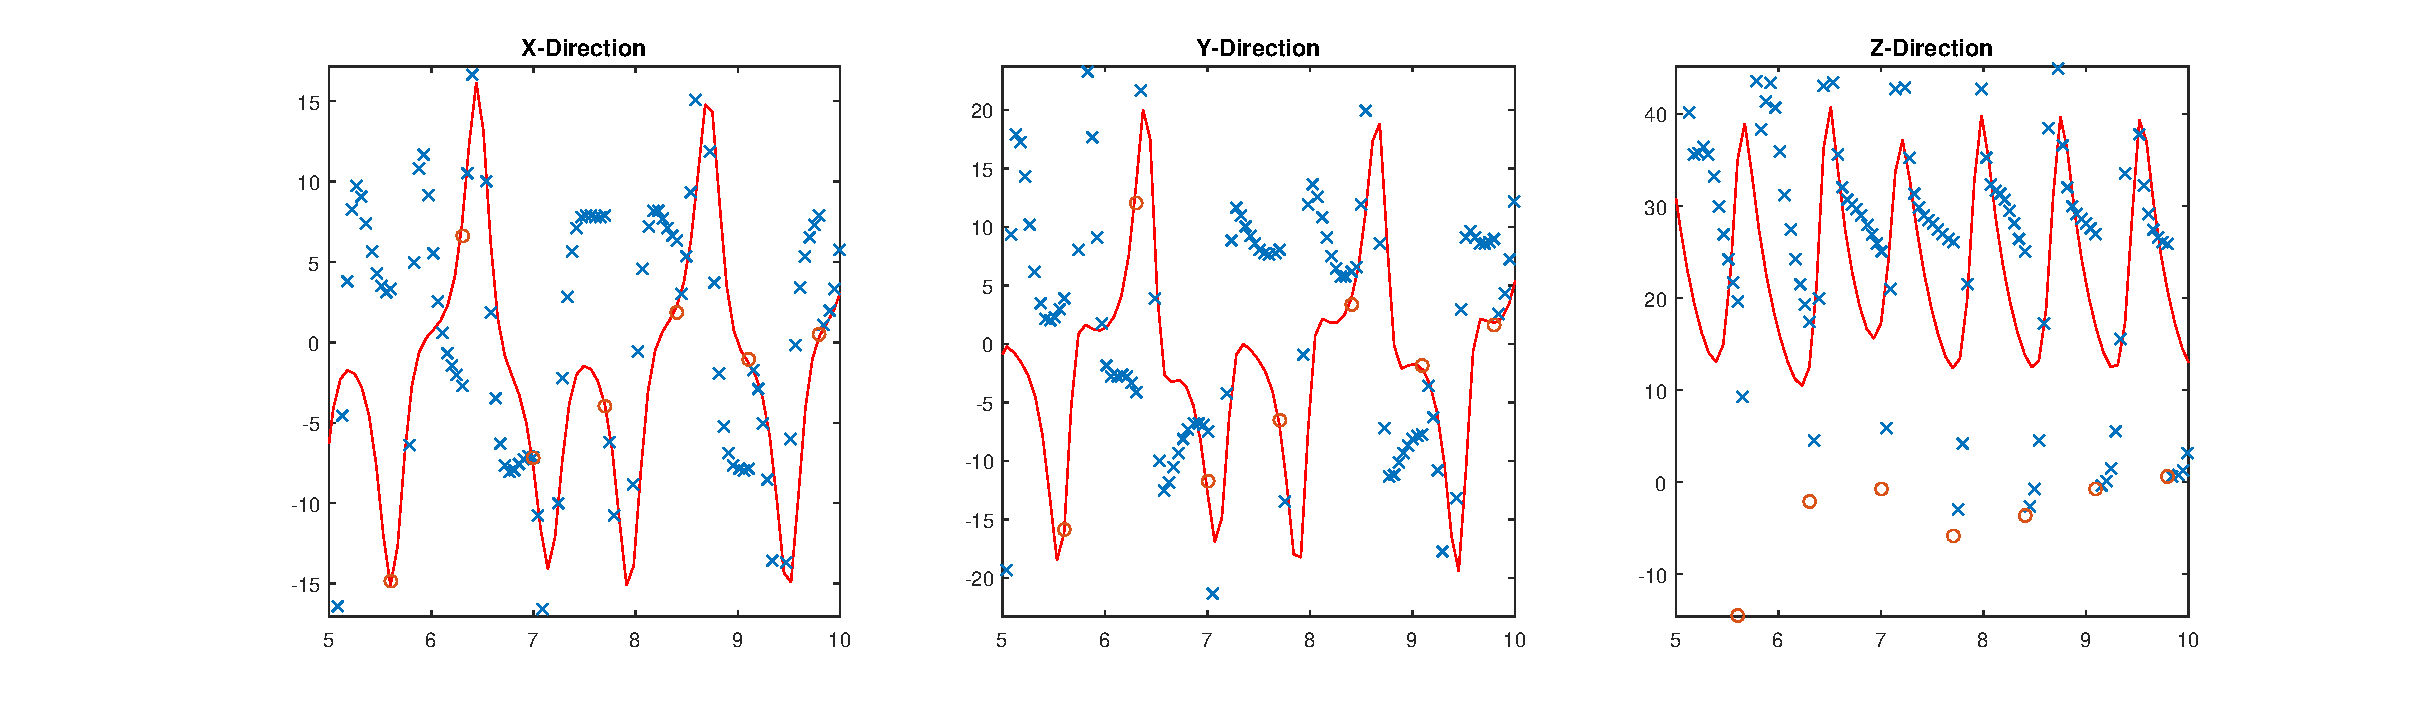
\includegraphics[width=\hsize]{kalman/figures/H3R10S1.eps}
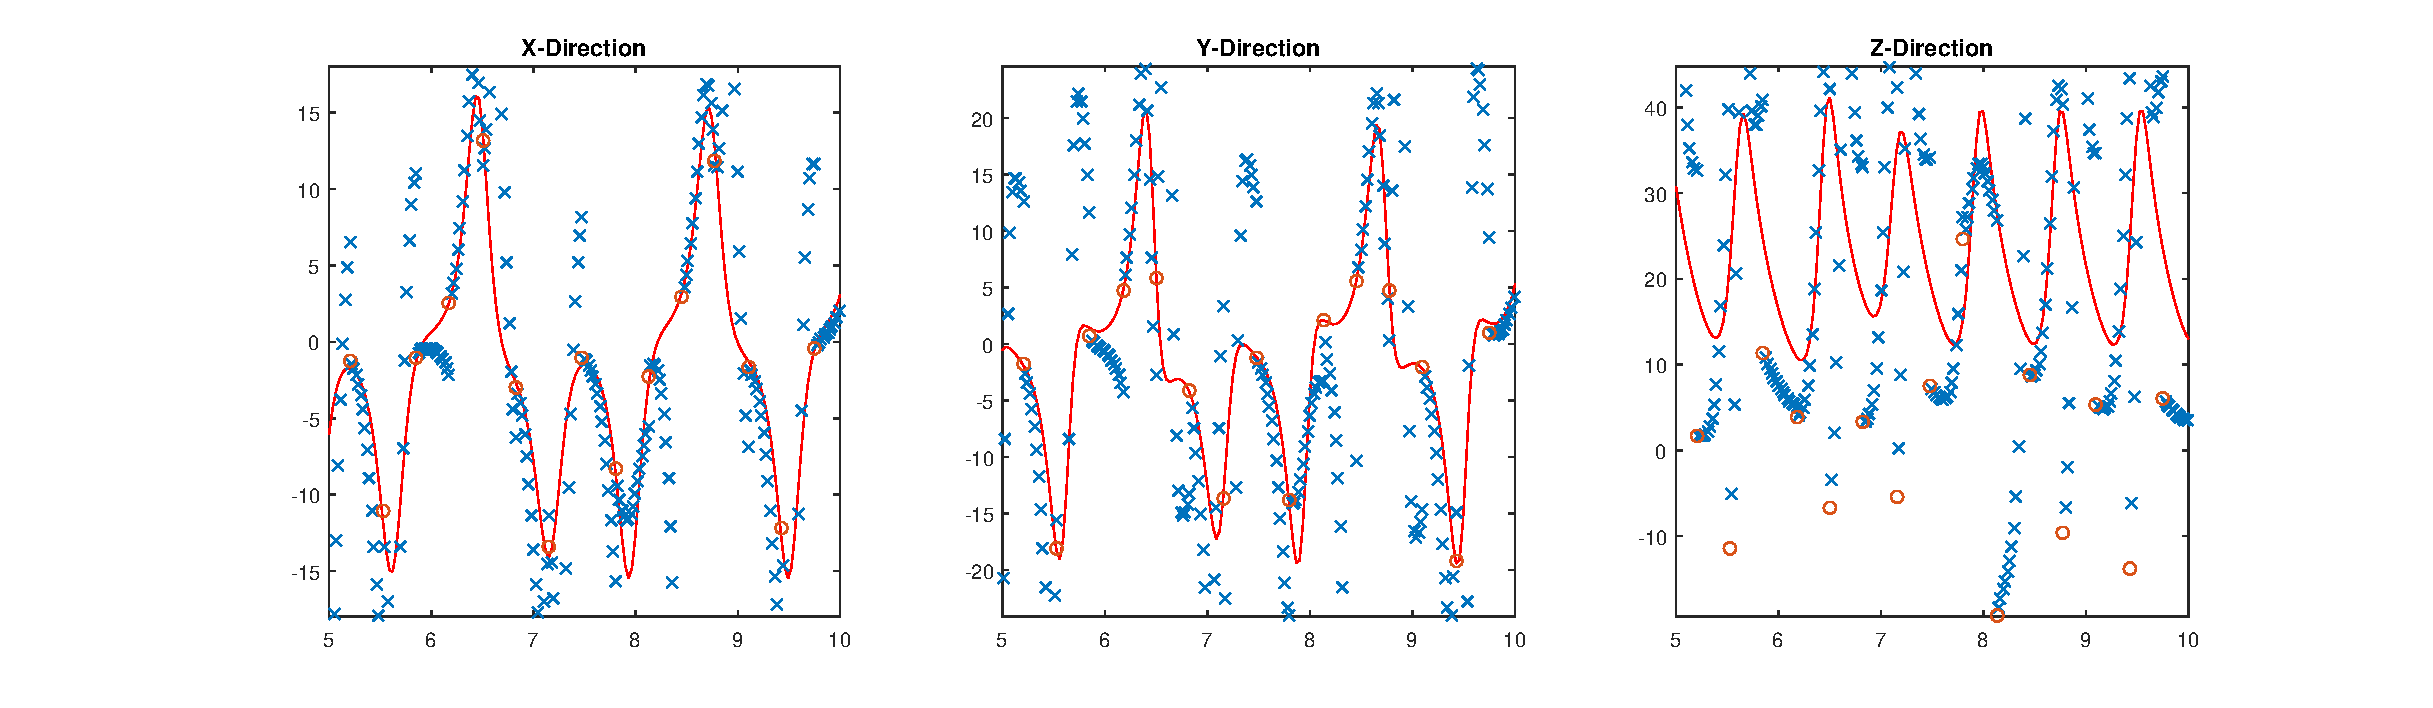
\includegraphics[width=\hsize]{kalman/figures/H3R20S2.eps}
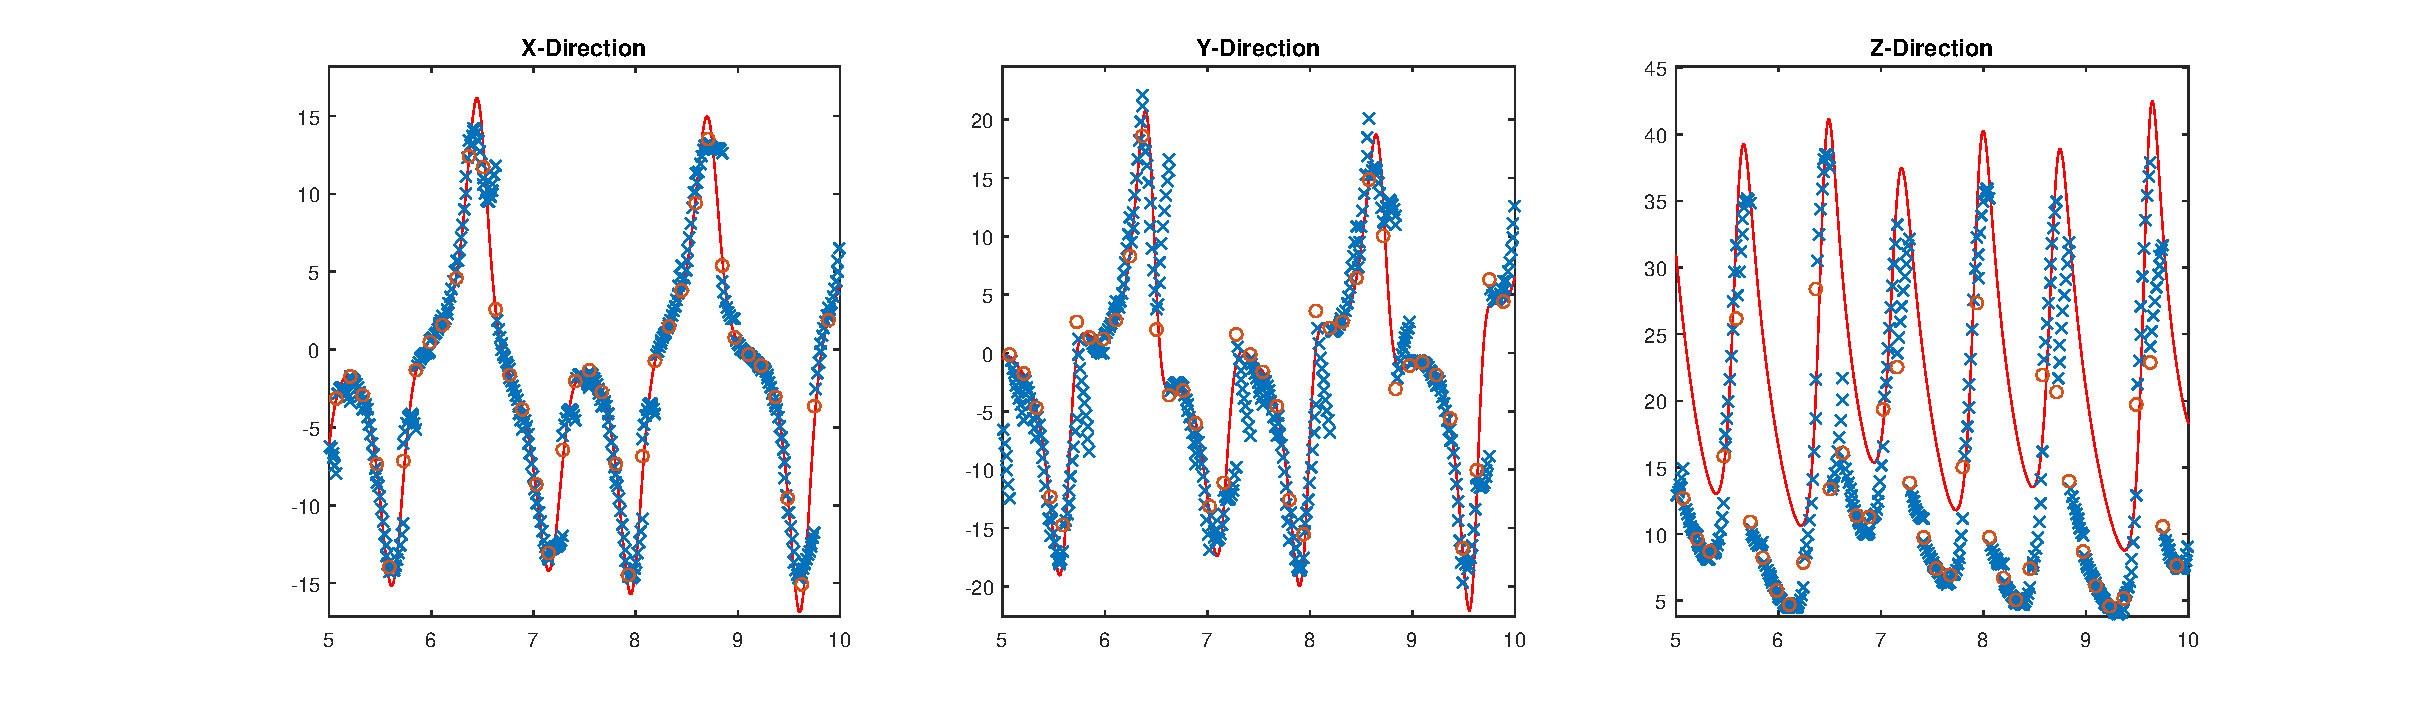
\includegraphics[width=\hsize]{kalman/figures/H3R05S5.eps}
\caption{Messmatrix H3 mit S=1, F=10 (oben), S=2 und F=20 (mitte) und S=5 und F=5 (unten)}
\label{skript:H3}
\end{figure}

Liegen wie mit $H4$ in Abbildung \ref{skript:H4} lediglich Werte f"ur $X$ und $Z$ vor, reicht dies nicht mehr f"ur eine Rekonstruktion der Realit"at. Die Simulationen liegen, abgesehen von den Z Werten, "ofters daneben, als dass sie die Drehrichtung richtig angeben. Eine Erh"ohung der Messkadenz oder genaueres Messen hilft nicht, die Vorhersagen zu verbessern. Dies deshalb, da das $Y$ relevante Informationen "uber das Gesamtsystem enth"alt.
Da die Messwerte f"ur $X$ und $Z$ zur Verf"ugung stehen, korrigiert der Filter diese trotzdem richtig.
Die Rekonstruktion der Z Werte scheint unter Umst"nden m"oglich zu sein, da kein chaotisches Verhalten vorliegt und daf"ur weniger Werte zur Verf"ung stehen m"ussen.

\begin{figure}
\centering
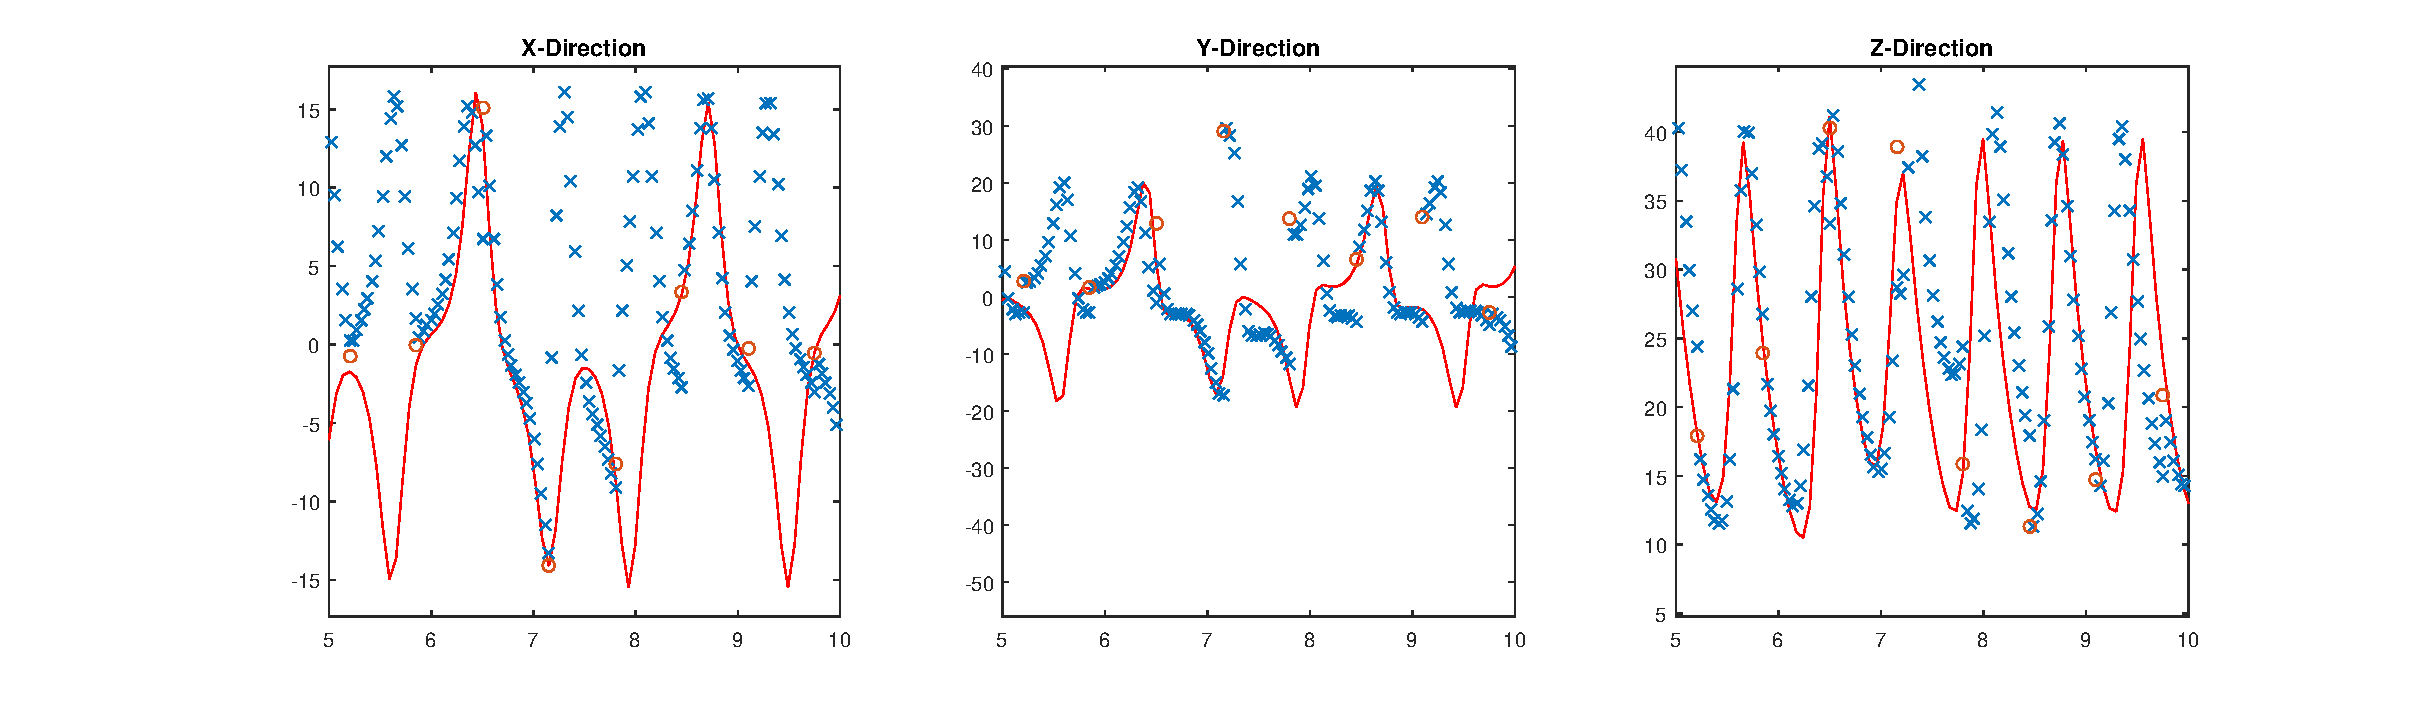
\includegraphics[width=\hsize]{kalman/figures/H4R10S1.eps}
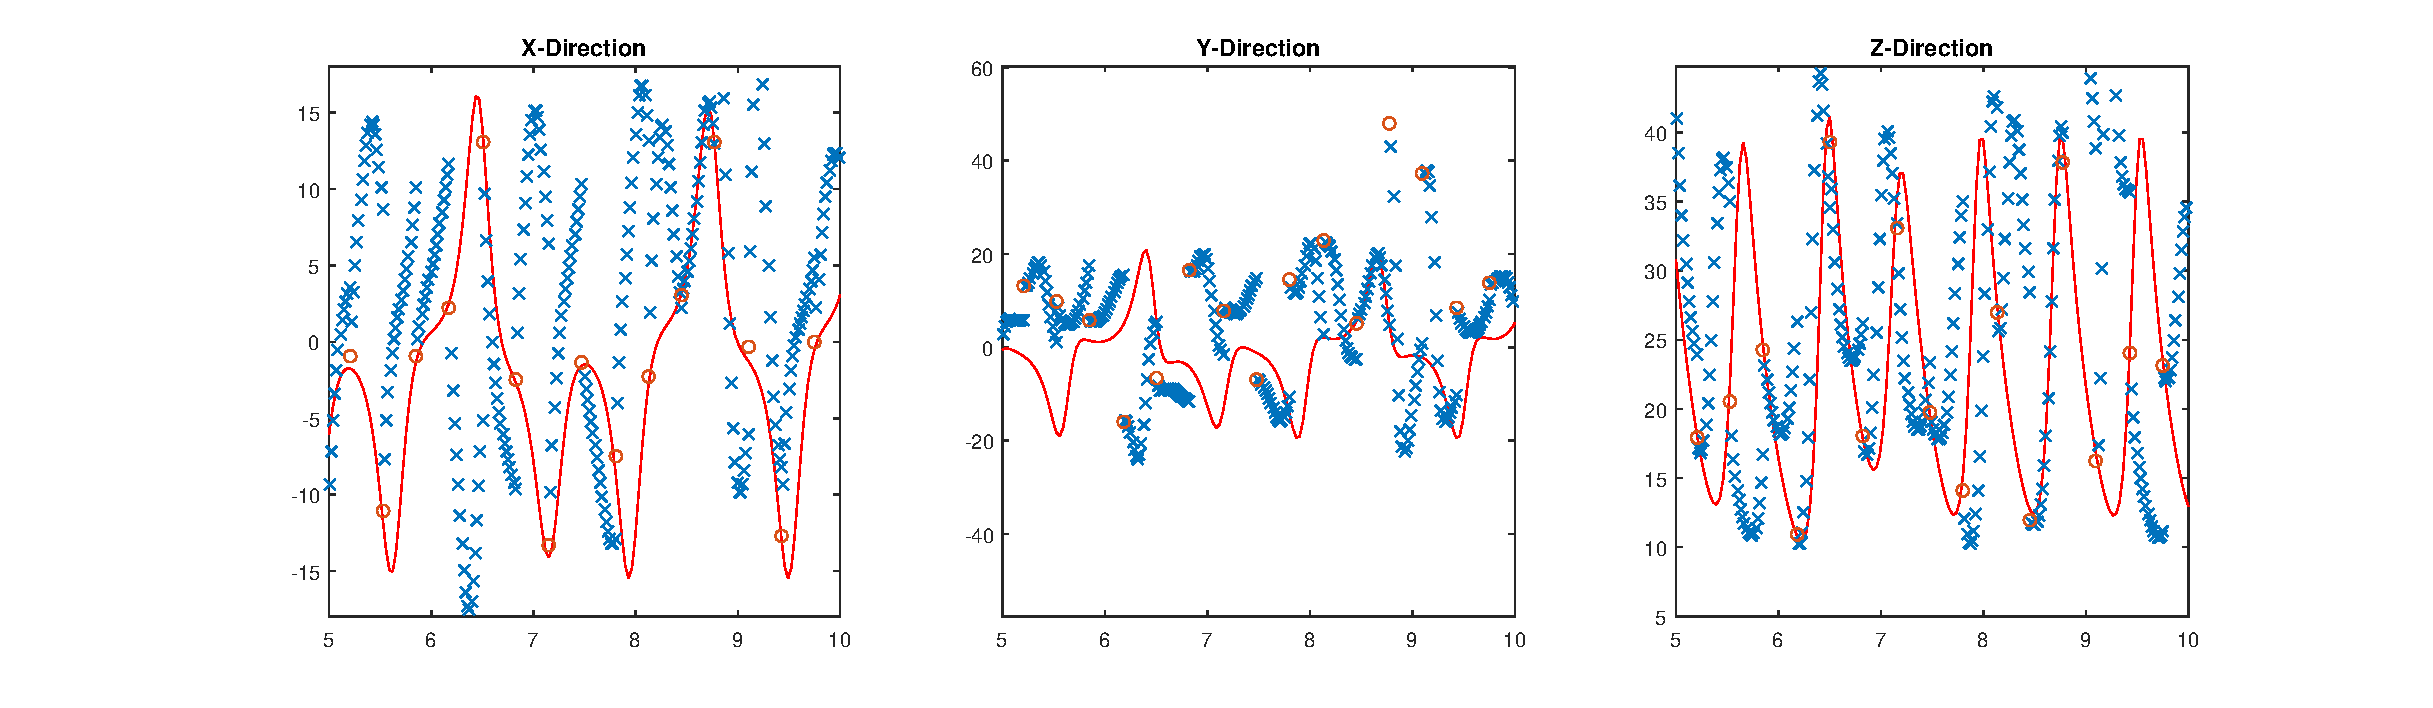
\includegraphics[width=\hsize]{kalman/figures/H4R20S2.eps}
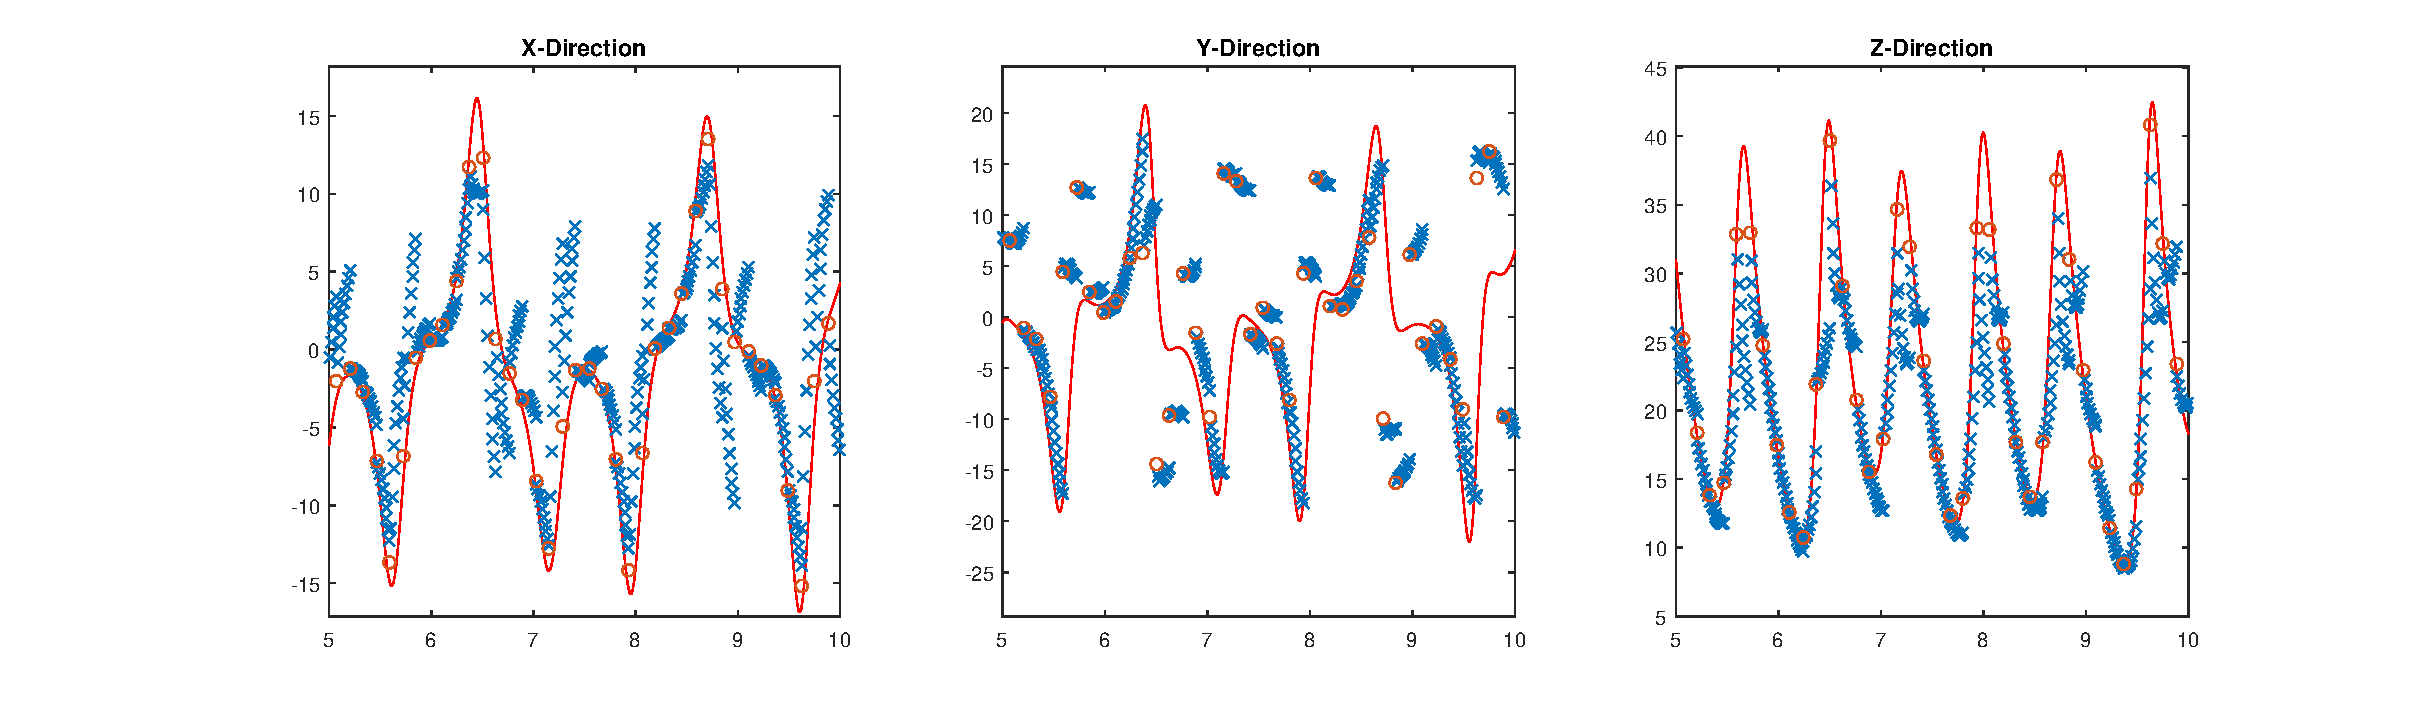
\includegraphics[width=\hsize]{kalman/figures/H4R05S5.eps}
\caption{Messmatrix H4 mit S=1, F=10 (oben), S=2 und F=20 (mitte) und S=5 und F=5 (unten)}
\label{skript:H4}
\end{figure}

\section{Schlussfolgerung}
\rhead{Schlussfolgerung}

Erkenntnisse:\\

Fehlender Messwert für Z und trotzdem brauchbare Vorhersagen.

Extrem chaotisches Verhalten bei marginalen Aenderungen der Parameter, fast egal welcher, und so sehr schwierig Simulationen genau nachzuvollziehen. Die Tendenzen scheinen aber auch mit theoretischen Überlegungen übereinzustimmen.

\printbibliography[heading=subbibliography]
\end{refsection}
